\chapter{Contextualización}
\minitoc
\label{chap:contextualizacion}
\vspace{0.5cm}

%%%%%%%%%%%%%%%%%%%%%%%%%%%%%%%%%%%%%%%%%%%%%%%%%%%%%%%%%%%%%%%%%%%%%%%%%%%%%%%%
% Objetivo: Contar cómo estaba la situación antes de empezar,                  %
%           todo lo que se hizo para familiarizarse con las tecnologías,       %
%           casarlas, etc.                                                     %
%%%%%%%%%%%%%%%%%%%%%%%%%%%%%%%%%%%%%%%%%%%%%%%%%%%%%%%%%%%%%%%%%%%%%%%%%%%%%%%%

\lettrine{A}{ntes} de entrar de cheo no corpo do proxecto, é preciso
contextualizar o mesmo desde varios puntos de vista (histórico, técnico,
estado da arte), coa finalidade de sentar as bases para a súa correcta
comprensión a posteriori.

\section{A gaita galega}

A gaita galega é un instrumento de vento madeira propio de Galicia, norte de
Portugal, occidente de Asturias e o Bierzo. É o símbolo por excelencia da
música tradicional galega \cite{WikipediaGaitaGalega}.

 \subsection{Breve percorrido histórico}

 A gaita de fol xorde hai aproximadamente 2000 anos cando alguén engadiu un
 fol, é dicir, un depósito flexible para o aire apertado debaixo do brazo, aos
 dous tubos sonoros que antes se tocaban directamente coa boca (clarinetes e
 óboes duplos -\ref{figura:CantigasSantaMariaClarinetesOboesDuplos}-); así
 xurdiron as gaitas de fol.

 \begin{figure}[htbp]
  \centering
  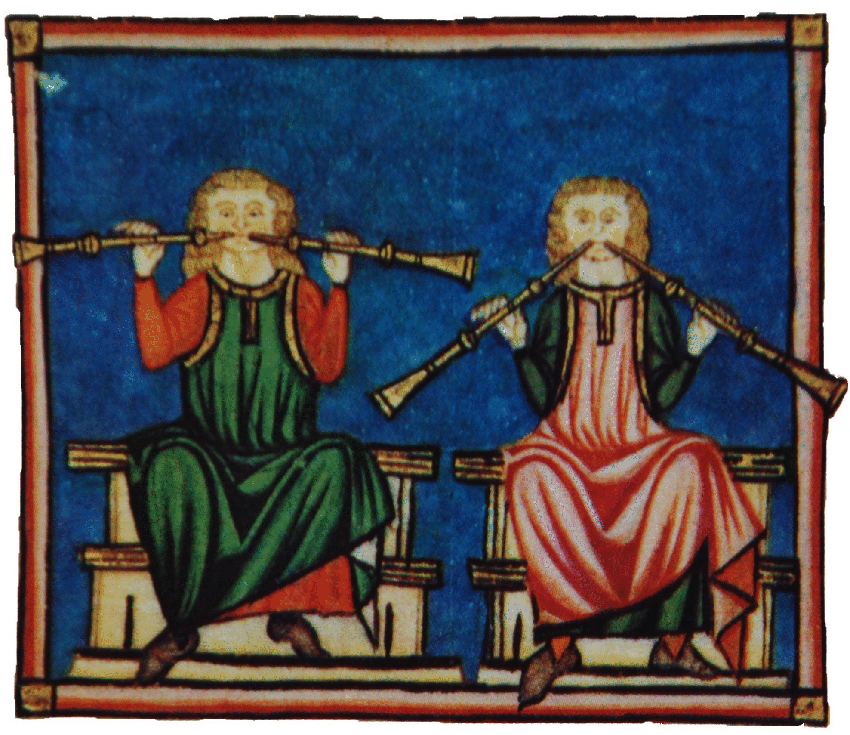
\includegraphics[scale=0.2,keepaspectratio=true]{./imagenes/cantigas-santa-maria-clarinetes-oboes-duplos.png}
  % cantigas-santa-maria-clarinetes-oboes-duplos.png: 850x735 pixel, 72dpi, 29.98x25.93 cm, bb=0 0 850 735
  \caption[Clarinetes/óboes duplos nas Cantigas de Santa María]{Representación de clarinetes/óboes duplos nas Cantigas de Santa María (s. XIII) \cite{CantigasSantaMariaClarinetesOboesDuplos}}
  \label{figura:CantigasSantaMariaClarinetesOboesDuplos}
 \end{figure}

 Antes do século XII carecemos practicamente de información iconográfica ou
 escrita que nos permita saber que aconteceu coa gaita de fol desde a invención
 do fol. Non entanto, a partir deste momento comeza a ser abundante a
 información, sobre todo a iconográfica, o que indica que a gaita de fol foi un
 importante instrumento musical, empregado tanto polas clases sociais
 superiores como polo pobo \cite{AGGGaitaGalega}. \\

 As primeiras representacións gráficas da gaita galega son de mediados do
 século XIII. Contaba entón de fol, punteiro e soprete, sen roncón (véxase o
 seguinte apartado). Coincidindo co desenvolvemento da polifonía,
 engadíronselle os bordóns e na segunda metade do XIII e no XIV aparece xa cun
 roncón, con dous, ou mesmo sen ningún (figura
 \ref{figura:CantigasSantaMariaGaitaGalega}). Nun principio, este tiña forma
 abucinada e posteriormente tomou a forma de copa.

 \begin{figure}[htbp]
  \centering
  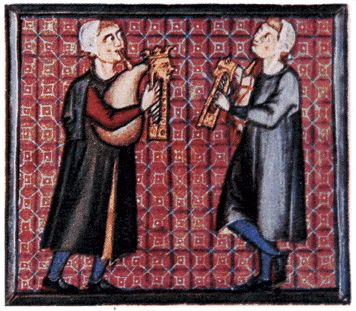
\includegraphics[scale=0.5,keepaspectratio=true]{./imagenes/cantigas-santa-maria-gaita-galega.jpg}
  % cantigas-santa-maria-gaita-galega.jpg: 356x311 pixel, 72dpi, 12.56x10.97 cm, bb=0 0 356 311
  \caption[Gaita galega nas Cantigas de Santa María]{Representación dunha gaita galega nas Cantigas de Santa María (s. XIII) \cite{WikipediaGaitaGalega}}
  \label{figura:CantigasSantaMariaGaitaGalega}
 \end{figure}

 Na segunda metade do século XIX introduciuse un chillón como apoio ó punteiro,
 colocado a carón deste. Ben entrado o século XX apareceu unha ronqueta, máis
 pequena que o segundo bordón dos séculos anteriores
 \cite{WikipediaGaitaGalega}.

 \subsection{Constitución}

 A gaita galega actual componse ou pode constar de \cite{WikipediaGaitaGalega}
 (figura \ref{figura:BrunoVillamorPartesGaitaGalega}):

 \begin{figure}[htbp]
  \centering
  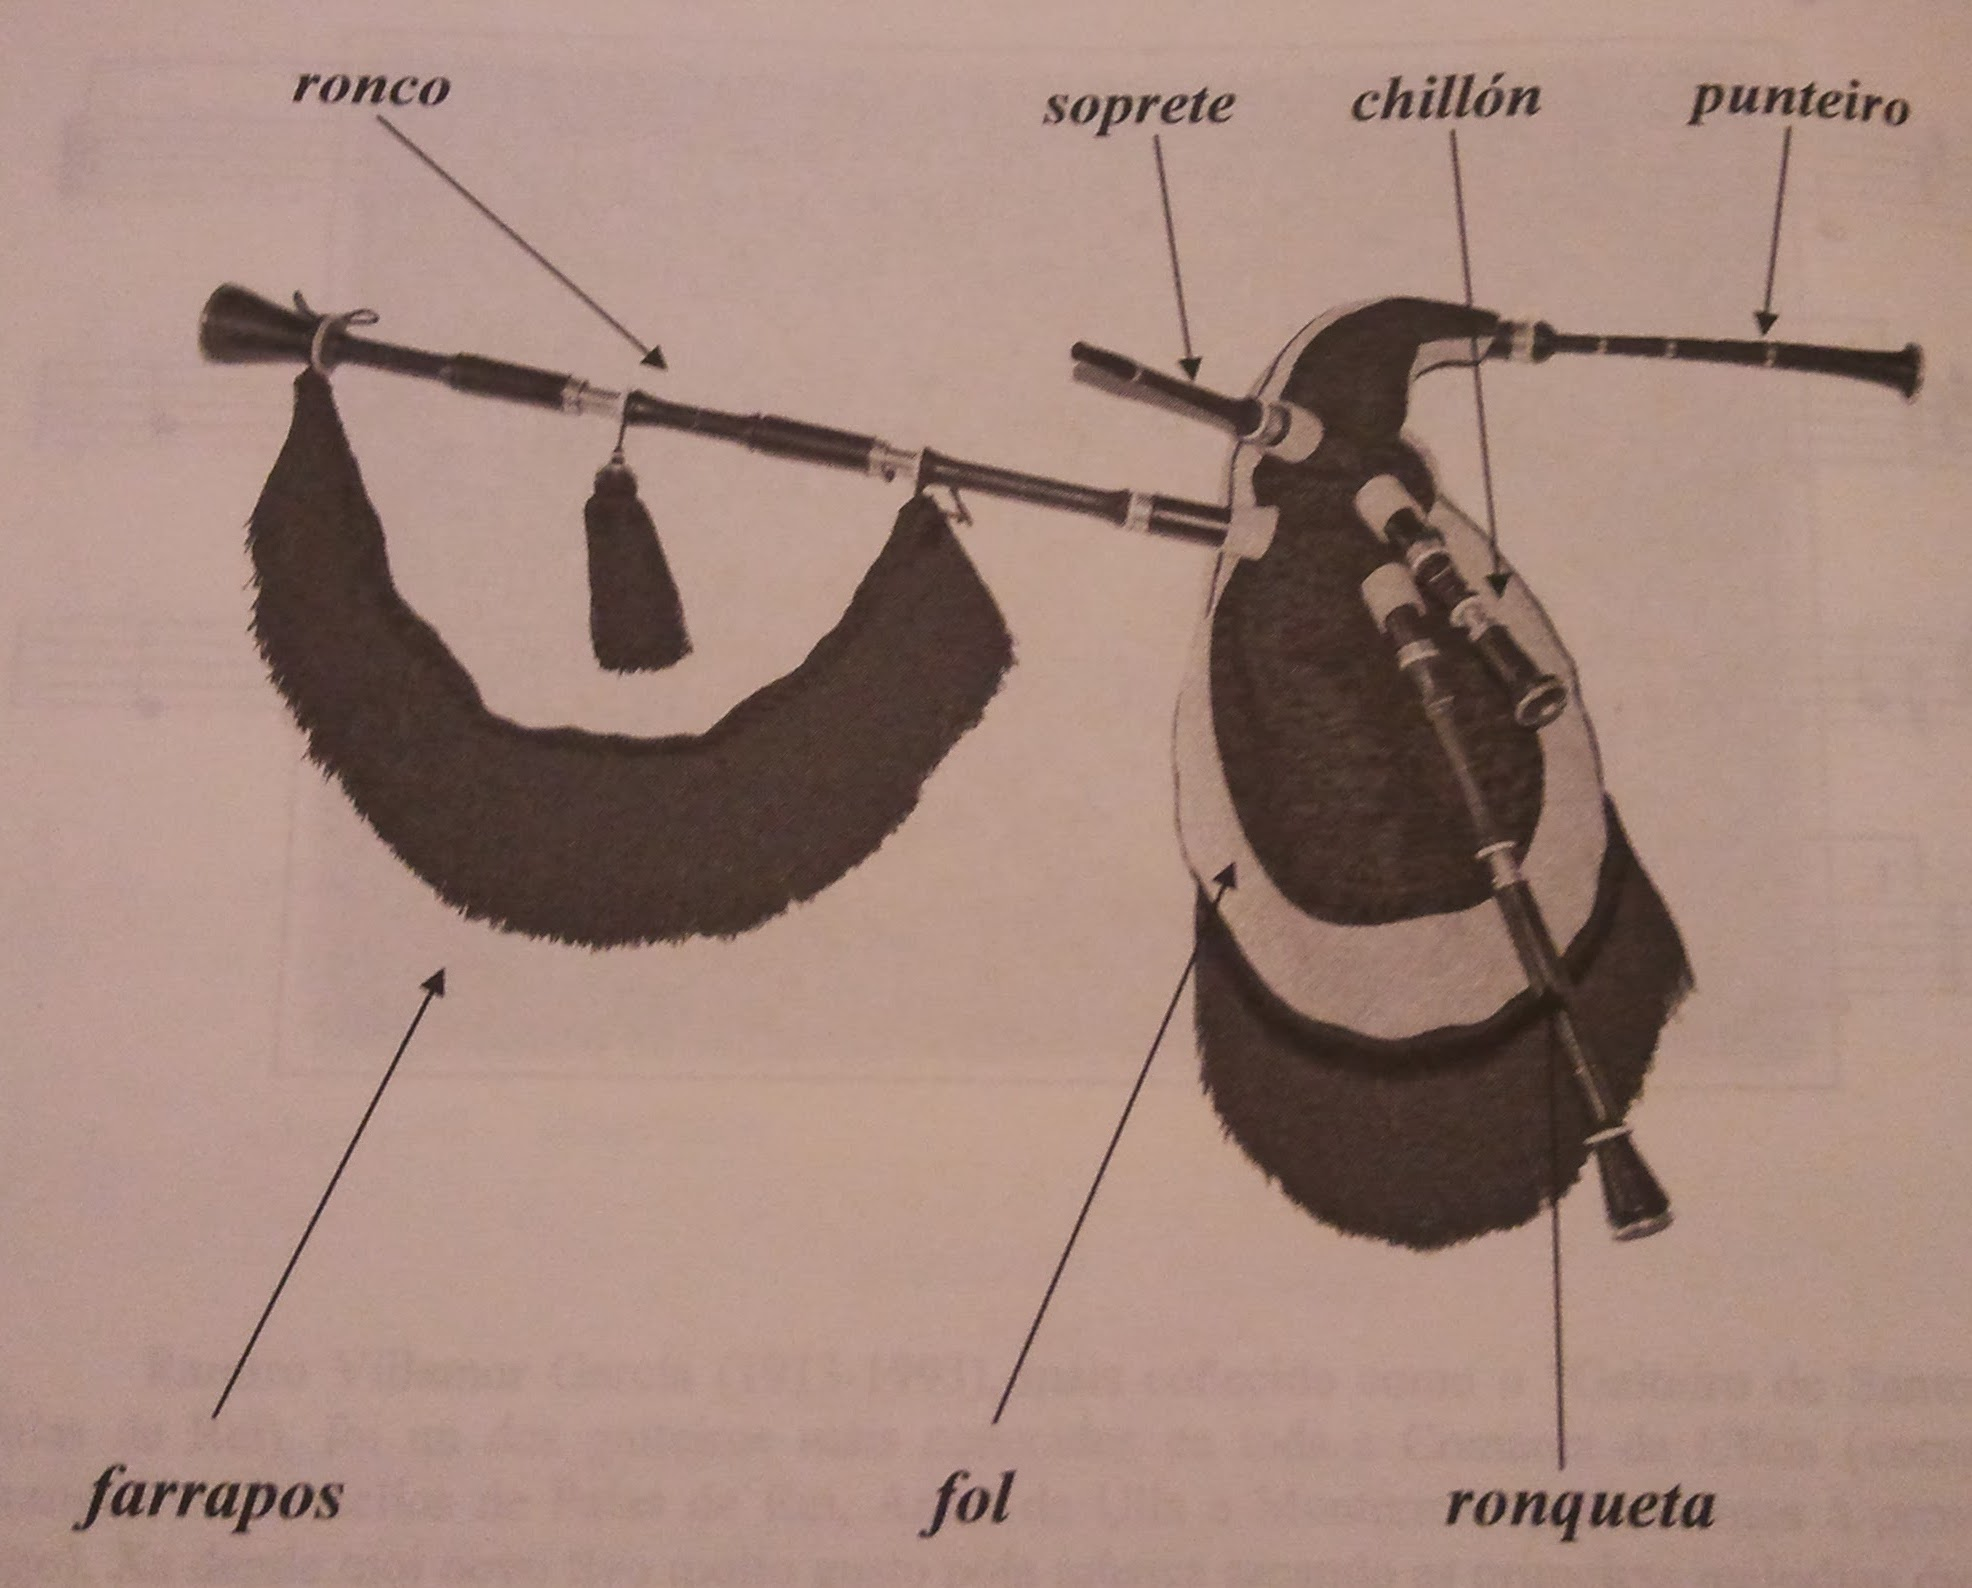
\includegraphics[scale=0.1,keepaspectratio=true]{./imagenes/bruno-villamor-partes-gaita-galega.jpg}
  % bruno-villamor-partes-gaita-galega.jpg: 1972x1588 pixel, 72dpi, 69.57x56.02 cm, bb=0 0 1972 1588
  \caption[Partes dunha gaita galega]{Partes dunha gaita galega \cite{BrunoVillamorCaderno15}}
  \label{figura:BrunoVillamorPartesGaitaGalega}
 \end{figure}

 \begin{itemize}
  \item Un \textbf{soprete}, co que se introduce o aire no fol.
  \item Un \textbf{fol}, onde se almacena o aire que fai que soe o instrumento.
  \item Un \textbf{punteiro}, o tubo cónico que sae polo frontal do fol e que é
        o que produce a melodía principal en base á colocación dos dedos.
  \item Un \textbf{ronco} ou \textbf{roncón}, o tubo que se apoia sobre o ombro
        do gaiteiro, que soa na mesma tonalidade que o punteiro, pero dúas
        oitavas máis grave.
  \item Unha \textbf{ronqueta}, o tubo que se apoia sobre o antebrazo dereito
        do gaiteiro, que soa na mesma tonalidade que o punteiro, pero unha
        oitava máis grave.
  \item Un \textbf{chillón} ou \textbf{ronquillo}, que sae do fol paralelo á
        ronqueta, que soa na dominante da tonalidade do punteiro e na mesma
        oitava.
 \end{itemize}

 \subsection{O punteiro}

 O punteiro é a parte máis importante e complexa da gaita galega
 \ref{figura:BrunoVillamorPunteiro}. \\

 \begin{figure}[htbp]
  \centering
  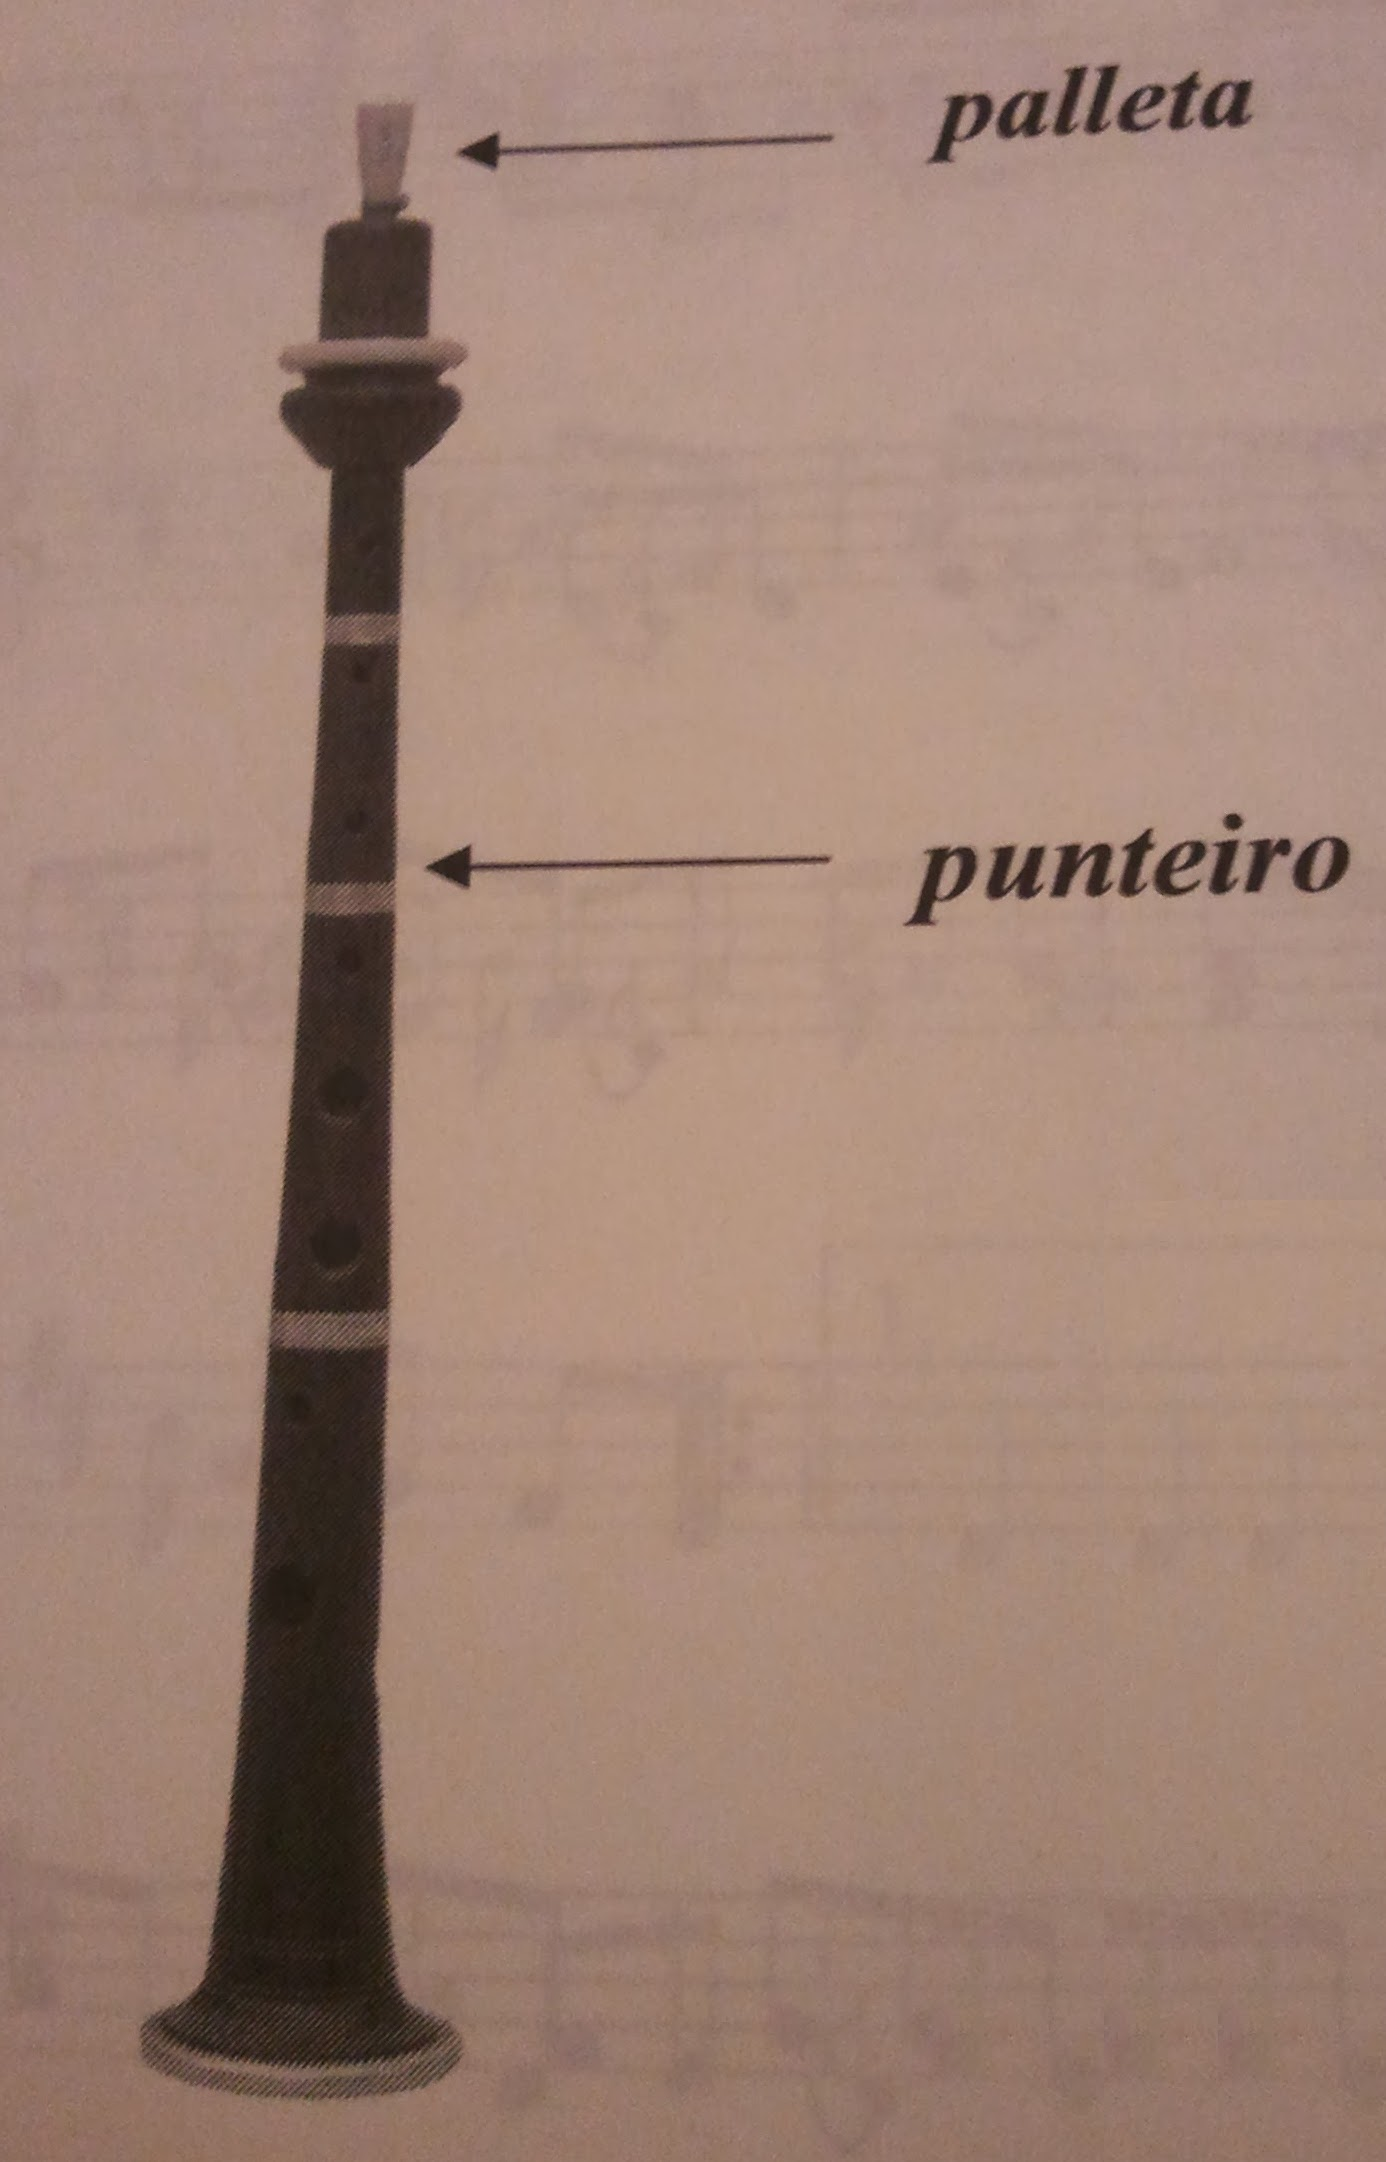
\includegraphics[scale=0.1,keepaspectratio=true]{./imagenes/bruno-villamor-punteiro.jpg}
  % bruno-villamor-punteiro.jpg: 1386x2162 pixel, 72dpi, 48.90x76.27 cm, bb=0 0 1386 2162
  \caption[Punteiro]{Punteiro \cite{BrunoVillamorCaderno15}}
  \label{figura:BrunoVillamorPunteiro}
 \end{figure}

 É o tubo sonoro no que facemos a melodía. É un tubo cónico de madeira onde se
 fan once (ou doce) buratos, dos cales tres permanecen sempre abertos (oídos do
 punteiro que serven para mellorar a afinación) e os restantes poden ficar
 abertos ou pechados polas xemas dos dedos segundo sexa necesario para acadar
 os diferentes sons e así poder crear unha melodía. \\

 \begin{figure}[htbp]
 \centering
 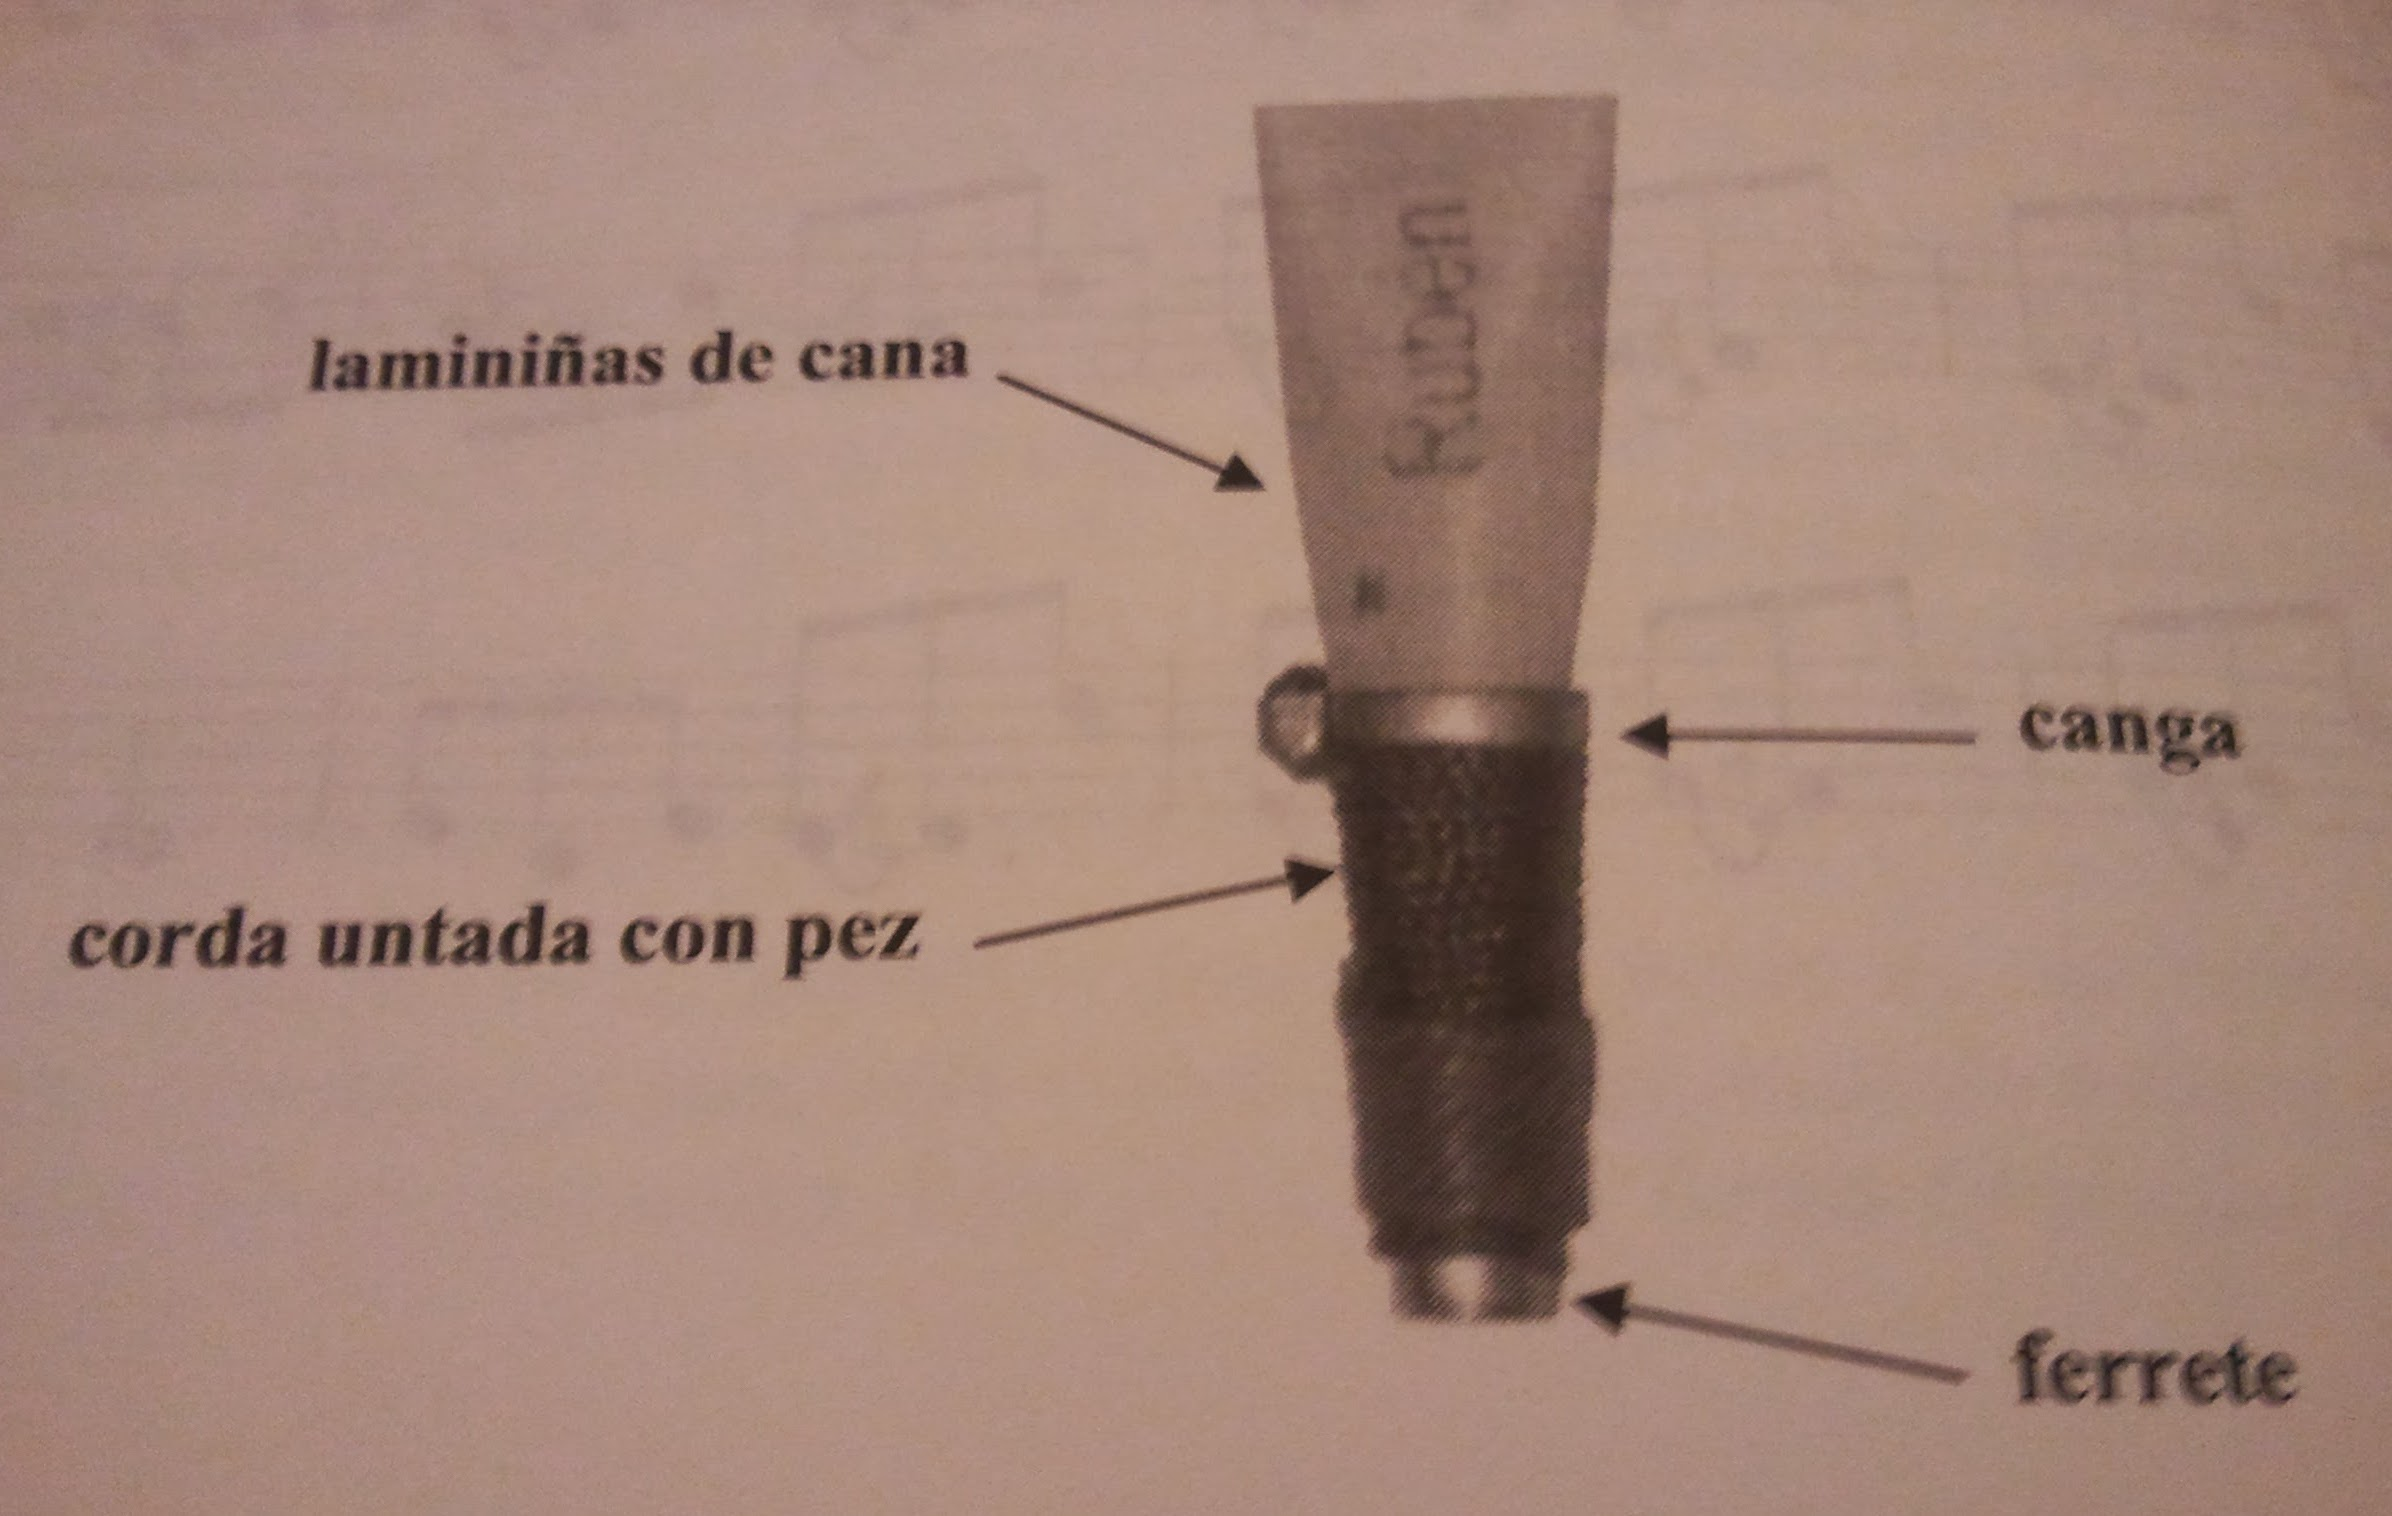
\includegraphics[scale=0.1,keepaspectratio=true]{./imagenes/bruno-villamor-palleta.jpg}
 % bruno-villamor-palleta.jpg: 2392x1516 pixel, 72dpi, 84.38x53.48 cm, bb=0 0 2392 1516
 \caption[Palleta]{Palleta \cite{BrunoVillamorCaderno15}}
 \label{figura:BrunoVillamorPalleta}
\end{figure}

 A \textbf{palleta} (figura \ref{figura:BrunoVillamorPalleta}) é o elemento que
 produce o son. Consiste en dúas laminiñas moi finas de cana de bambú que se
 colocan sobre dun tudel metálico que recibe o nome de ferrete (normalmente de
 latón ou cobre) que se amarran ó mesmo empregando corda untada con pez e un
 ariño metálico (normalmente arame de latón) coñecido co nome de canga. A
 calidade e singularidade do son do punteiro vese condicionada en gran medida
 pola calidade da palleta \cite{BrunoVillamorCaderno15}.

 \subsection{Os bordóns}

 Coñécense coma \textbf{bordóns} o conxunto de tubos sonoros que producen notas
 pedal\footnote{Na música tonal, unha nota pedal é unha nota sostida ou
 continua que se mantén mentres o resto da melodía segue avanzando.}. No caso
 da gaita galega, o ronco, a ronqueta e o chillón. \\

 \begin{figure}[htbp]
  \centering
  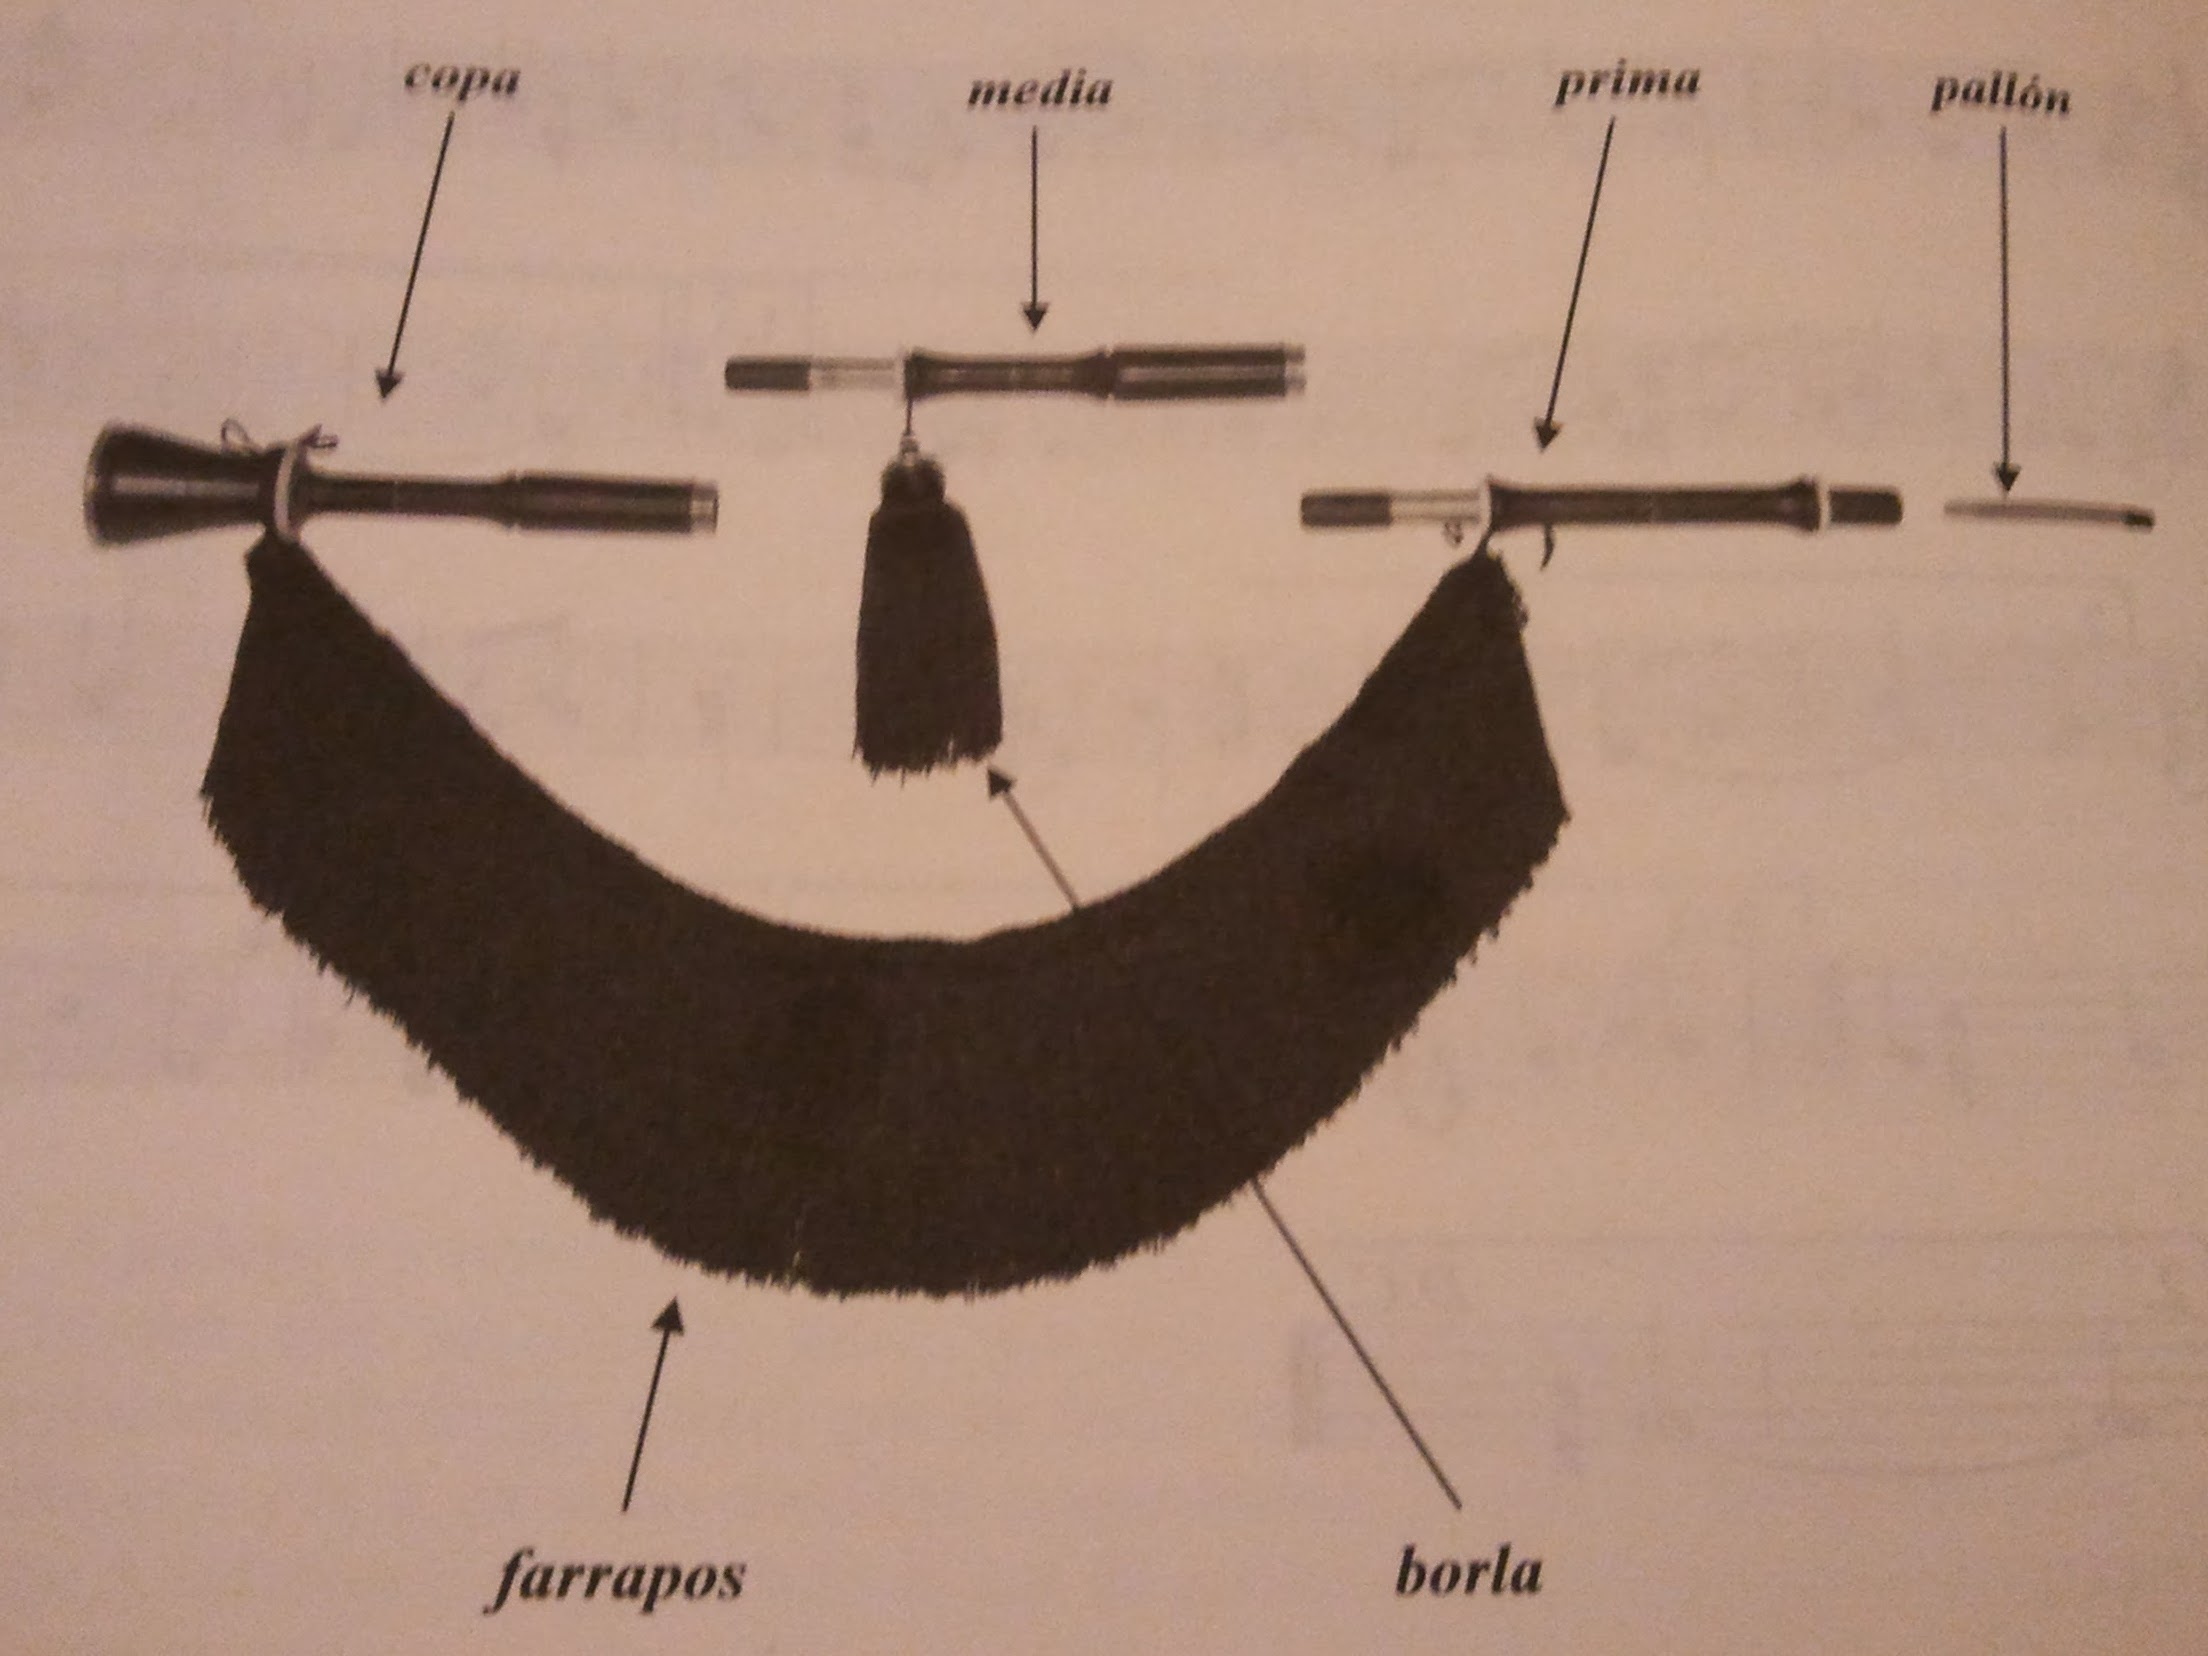
\includegraphics[scale=0.1,keepaspectratio=true]{./imagenes/bruno-villamor-ronco.jpg}
  % bruno-villamor-ronco.jpg: 2208x1656 pixel, 72dpi, 77.89x58.42 cm, bb=0 0 2208 1656
  \caption[Ronco]{Ronco \cite{BrunoVillamorCaderno15}}
  \label{figura:BrunoVillamorRonco}
 \end{figure}

 O \textbf{ronco} (figura \ref{figura:BrunoVillamorRonco}) é un tubo sonoro
 construído en madeira que se fai en tres partes (prima, media e copa) e que
 produce unha nota pedal. Está feito en tres partes para poder xogar coa súa
 lonxitude e así poder afinar co punteiro, sempre canto máis alonguemos o ronco
 máis grave será o seu son e canto máis o acurtemos máis agudo. O ronco afínase
 sobre a tónica do punteiro, e o seu son é dúas oitavas máis grave que o son
 deste. \\

 \begin{figure}[htbp]
  \centering
  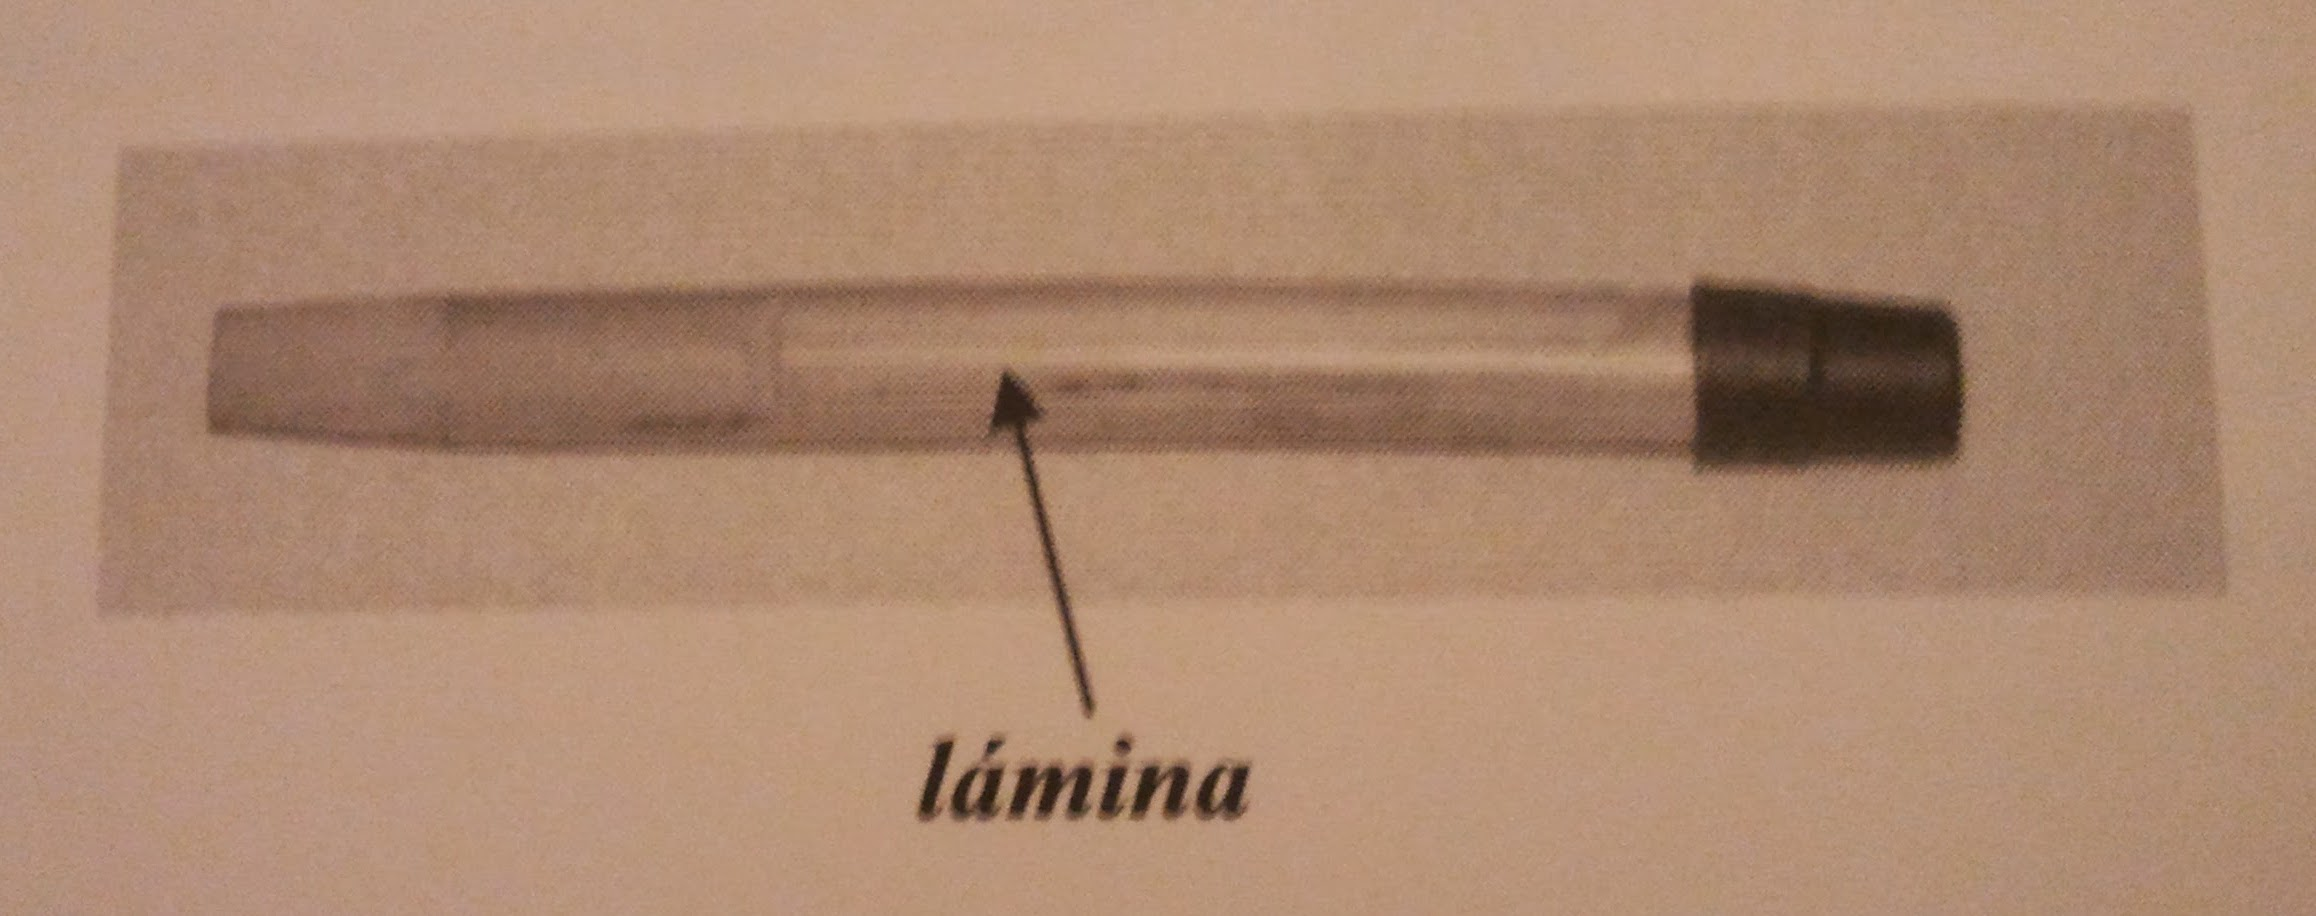
\includegraphics[scale=0.1,keepaspectratio=true]{./imagenes/bruno-villamor-pallon.jpg}
  % bruno-villamor-pallon.jpg: 2316x916 pixel, 72dpi, 81.70x32.31 cm, bb=0 0 2316 916
  \caption[Pallón]{Pallón \cite{BrunoVillamorCaderno15}}
  \label{figura:BrunoVillamorPallon}
 \end{figure}


 O son é producido polo \textbf{pallón} (\ref{figura:BrunoVillamorPallon}), que
 é un trociño de cana de bambú pechado por un dos seus extremos sobre o que se
 fai un corte oblicuo de non moita extensión. \\

 \begin{figure}[htbp]
  \centering
  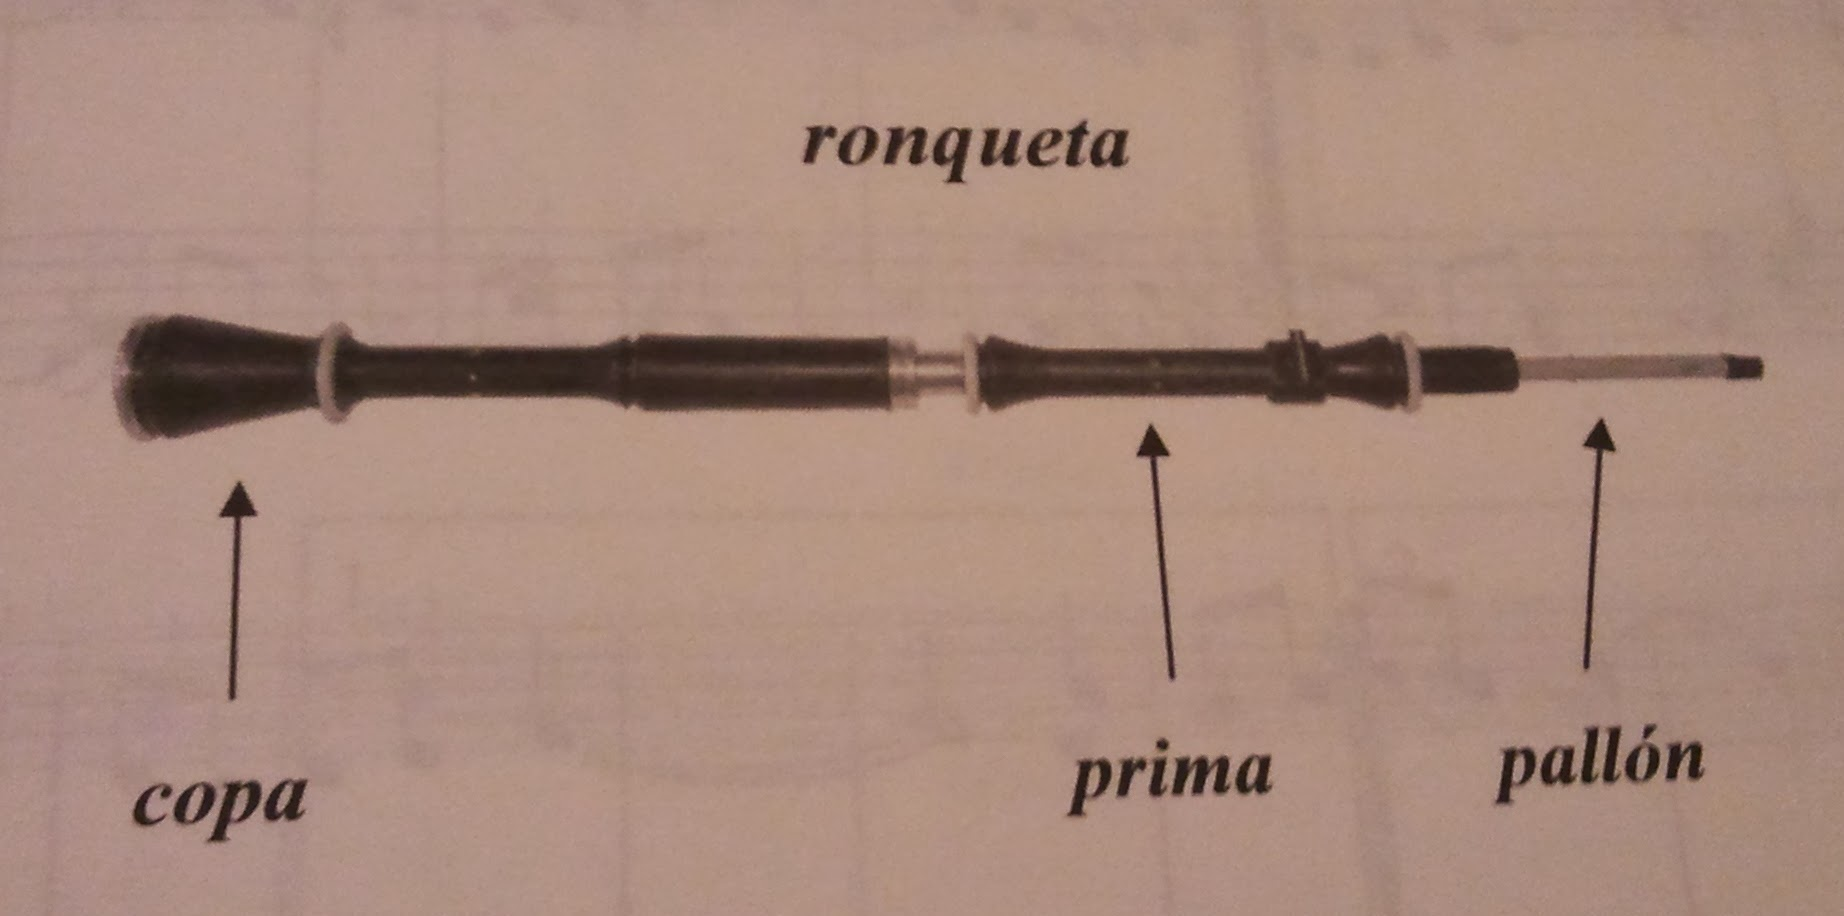
\includegraphics[scale=0.1,keepaspectratio=true]{./imagenes/bruno-villamor-ronqueta.jpg}
  % bruno-villamor-ronqueta.jpg: 2560x1920 pixel, 72dpi, 90.31x67.73 cm, bb=0 0 2560 1920
  \caption[Ronqueta]{Ronqueta \cite{BrunoVillamorCaderno15}}
  \label{figura:BrunoVillamorRonqueta}
 \end{figure}

 A \textbf{ronqueta} (figura \ref{figura:BrunoVillamorRonqueta}) é un tubo
 sonoro de madeira construído en dúas pezas (prima e copa). O son prodúceo un
 pallón de dimensións máis reducidas cas do pallón que utiliza o ronco. Afínase
 na tónica do punteiro e o seu son é unha oitava máis grave que o son do
 punteiro. Ó igual que o ronco mantén unha nota pedal. \\

 \begin{figure}[htbp]
  \centering
  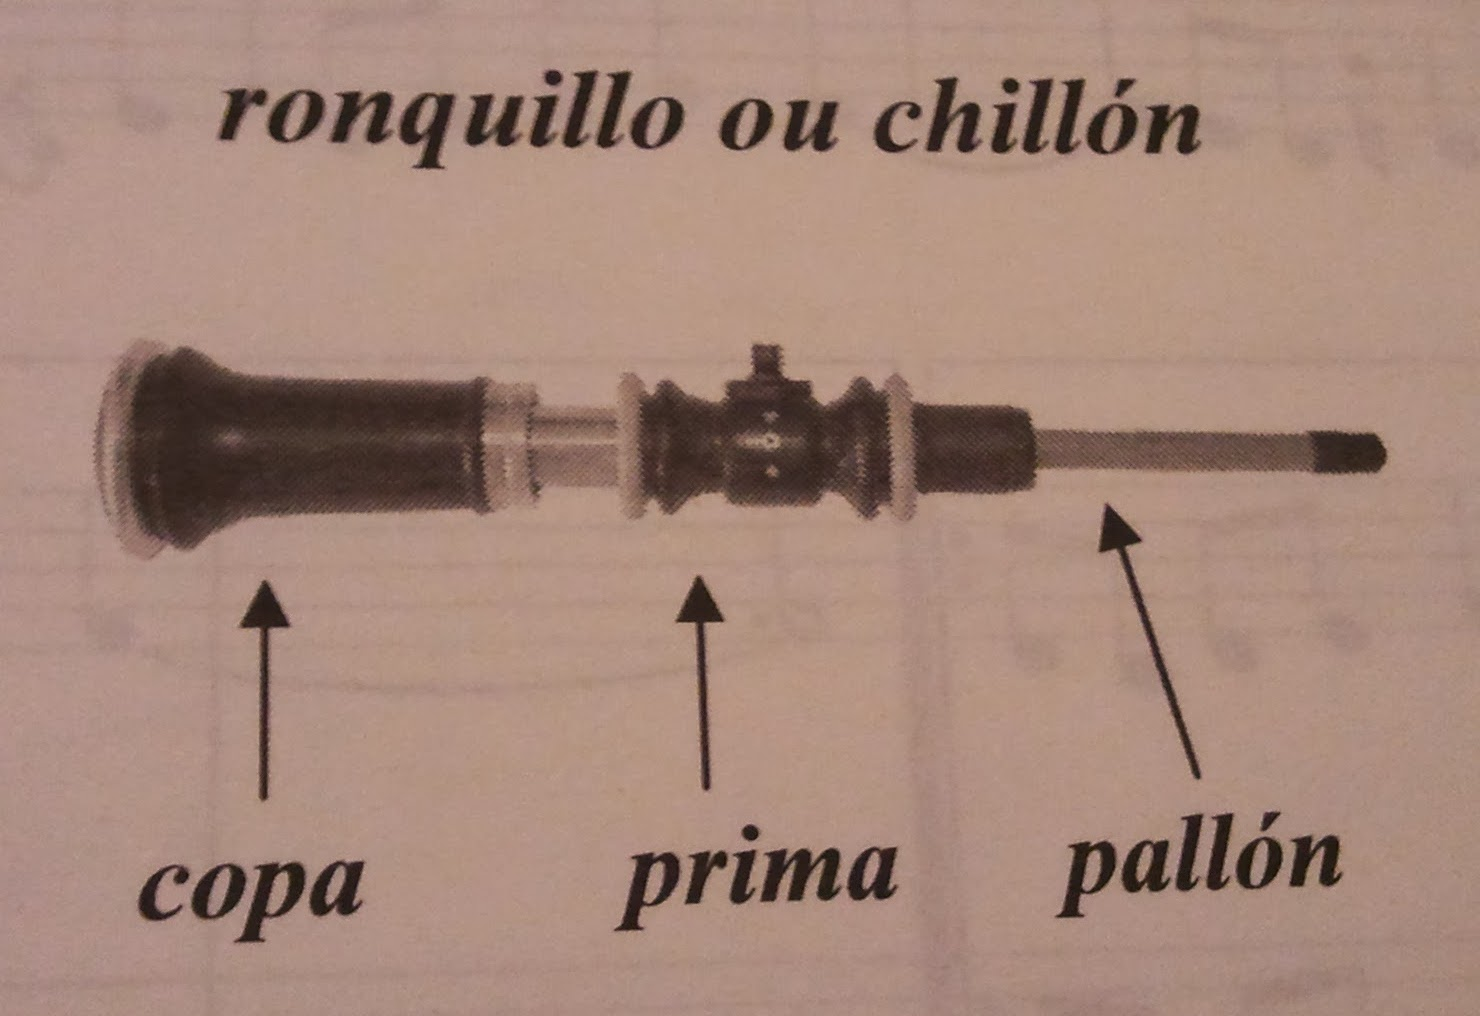
\includegraphics[scale=0.1,keepaspectratio=true]{./imagenes/bruno-villamor-chillon.jpg}
  % bruno-villamor-chillon.jpg: 1480x1016 pixel, 72dpi, 52.21x35.84 cm, bb=0 0 1480 1016
  \caption[Chillón]{Chillón \cite{BrunoVillamorCaderno15}}
  \label{figura:BrunoVillamorChillon}
 \end{figure}

 O \textbf{chillón} (figura \ref{figura:BrunoVillamorChillon}) é un tubo sonoro
 de madeira construído en dúas pezas só que de tamaño máis pequeno que as da
 ronqueta. O son pode estar producido por un pallón pequeniño ou por unha
 palleta (igual á que se emprega no punteiro), estes últimos son os verdadeiros
 chillóns aínda que na actualidade están quedando en desuso xa que a súa forte
 sonoridade tapa a melodía producida polo punteiro. Os chillóns que empregan
 pallón afínanse na dominante do punteiro e os que empregan palleta afínanse na
 tónica, estando ambos na oitava deste \cite{BrunoVillamorCaderno15}.

 \subsection{Dixitación}

 Defínese como \textbf{dixitación} da gaita galega a maneira concreta de
 colocación dos dedos sobre o punteiro. Tradicionalmente falando, existen dous
 modos de dixitación: \textit{aberto} e \textit{pechado}. \\

 No modo \textit{aberto} (figura \ref{figura:PabloCarpinteroDixitacionAberta})
 vanse erguendo os dedos ata a nota que se desexa facer soar. Este é o modo
 máis extendido a día de hoxe. \\

 \begin{figure}[htbp]
  \centering
  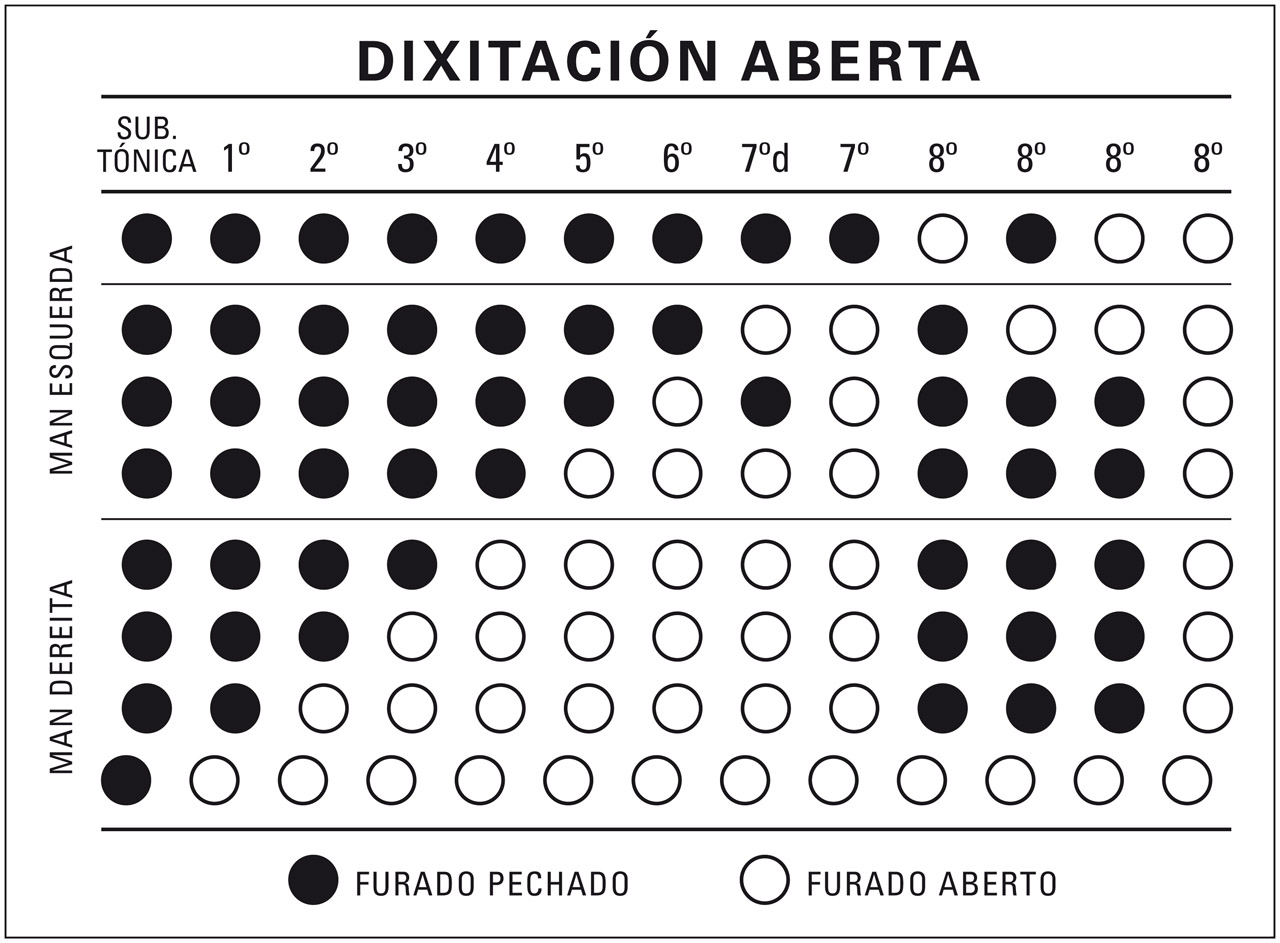
\includegraphics[scale=0.2,keepaspectratio=true]{./imagenes/pablo-carpintero-dixitacion-aberta.jpg}
  % pablo-carpintero-dixitacion-aberta.jpg: 1280x943 pixel, 300dpi, 10.84x7.98 cm, bb=0 0 307 226
  \caption[Dixitación aberta]{Dixitación aberta \cite{PabloCarpintero}}
  \label{figura:PabloCarpinteroDixitacionAberta}
 \end{figure}

 No modo \textit{pechado}
 (figura \ref{figura:PabloCarpinteroDixitacionPechada}) só se ergue o dedo que
 se corresponde coa nota que se quere facer soar. É de facer notar que existen
 diferentes modos de dixitación en pechado, pero a máis extendida no noso país
 é a que se amosa a continuación. \\

 \begin{figure}[htbp]
  \centering
  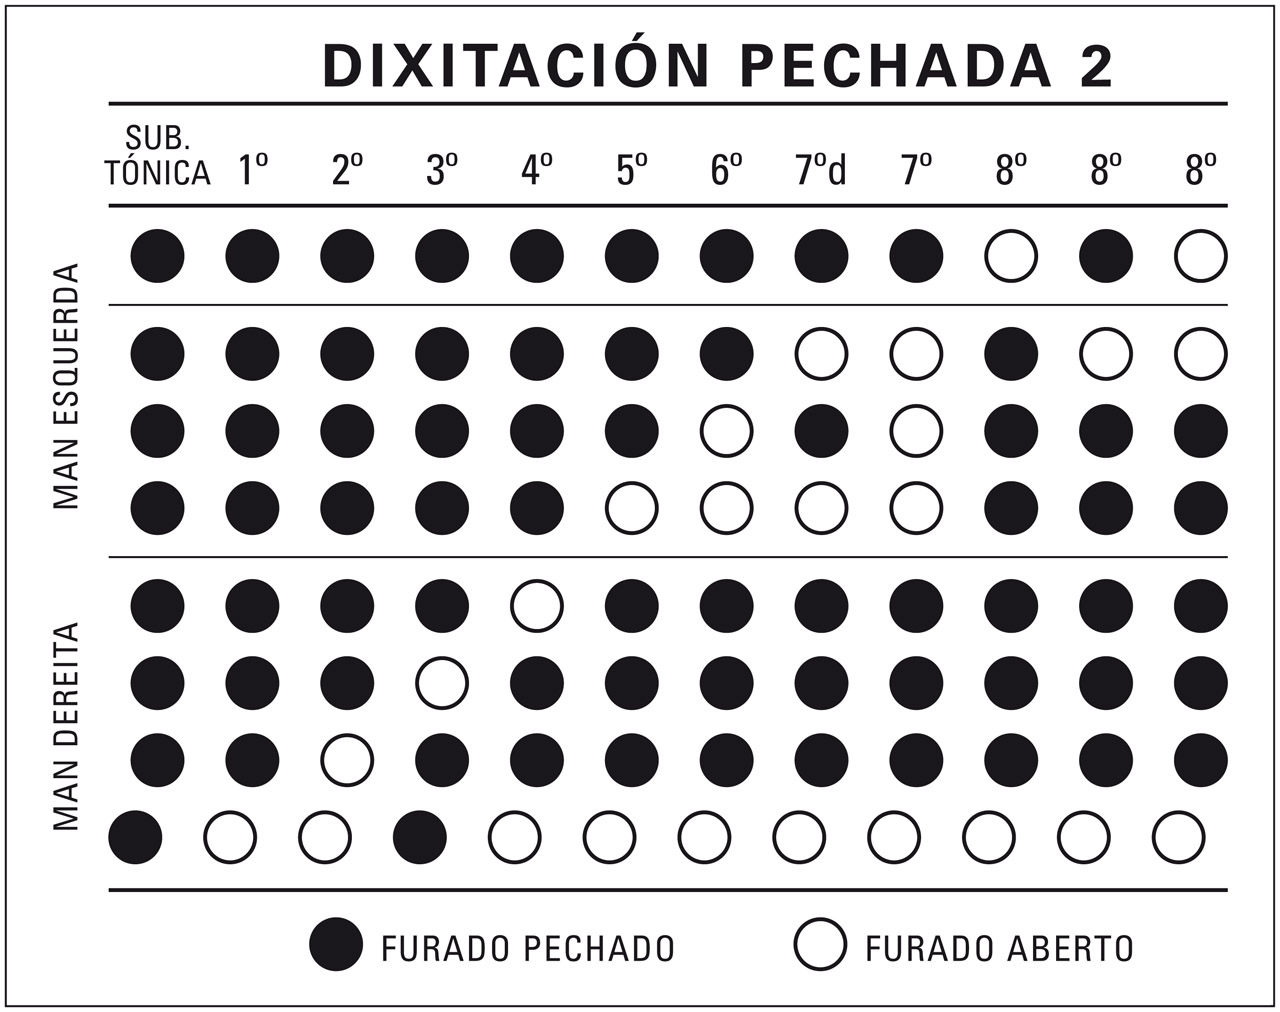
\includegraphics[scale=0.2,keepaspectratio=true]{./imagenes/pablo-carpintero-dixitacion-pechada-2.jpg}
  % pablo-carpintero-dixitacion-pechada-2.jpg: 1280x1012 pixel, 300dpi, 10.84x8.57 cm, bb=0 0 307 243
  \caption[Dixitación pechada]{Dixitación pechada \cite{PabloCarpintero}}
  \label{figura:PabloCarpinteroDixitacionPechada}
 \end{figure}

 \subsection{Tonalidade}

 Tradicionalmente podemos atopar por toda a xeografía galega gaitas afinadas en
 diferentes tonalidades, as cales reciben os seguintes nomes:

 \begin{itemize}
  \item Gaita grileira (afinada en Re).
  \item Gaita redonda (afinada en Do).
  \item Gaita tumbal (afinada en Si b).
 \end{itemize}

 A altura de son dun tubo sonoro varía en función da súa lonxitude e do seu
 calibre interno, de forma que canto maior sexan estes, máis grave será a
 afinación e canto menor sexan, máis aguda. Polo tanto, a gaita que maiores
 dimensións ten é a gaita tumbal e a que menores, a gaita grileira. \\

 Para unha maior facilidade de lectura represéntase exactamente igual na
 partitura unha melodía tocada por unha gaita grileira que por unha gaita
 tumbal ou por unha gaita redonda, indicando, iso si, ó comezo da peza, que
 gaita debemos empregar. Á hora de tocar con outros instrumentos debemos ser
 conscientes da diferenza que hai da representación escrita ó son real que
 producimos con cada gaita. A continuación amosáse a relación que existe entre
 ambas \cite{BrunoVillamorCaderno18} (figura
 \ref{figura:BrunoVillamorTonalidade}): \\

 \begin{figure}[htbp]
  \centering
  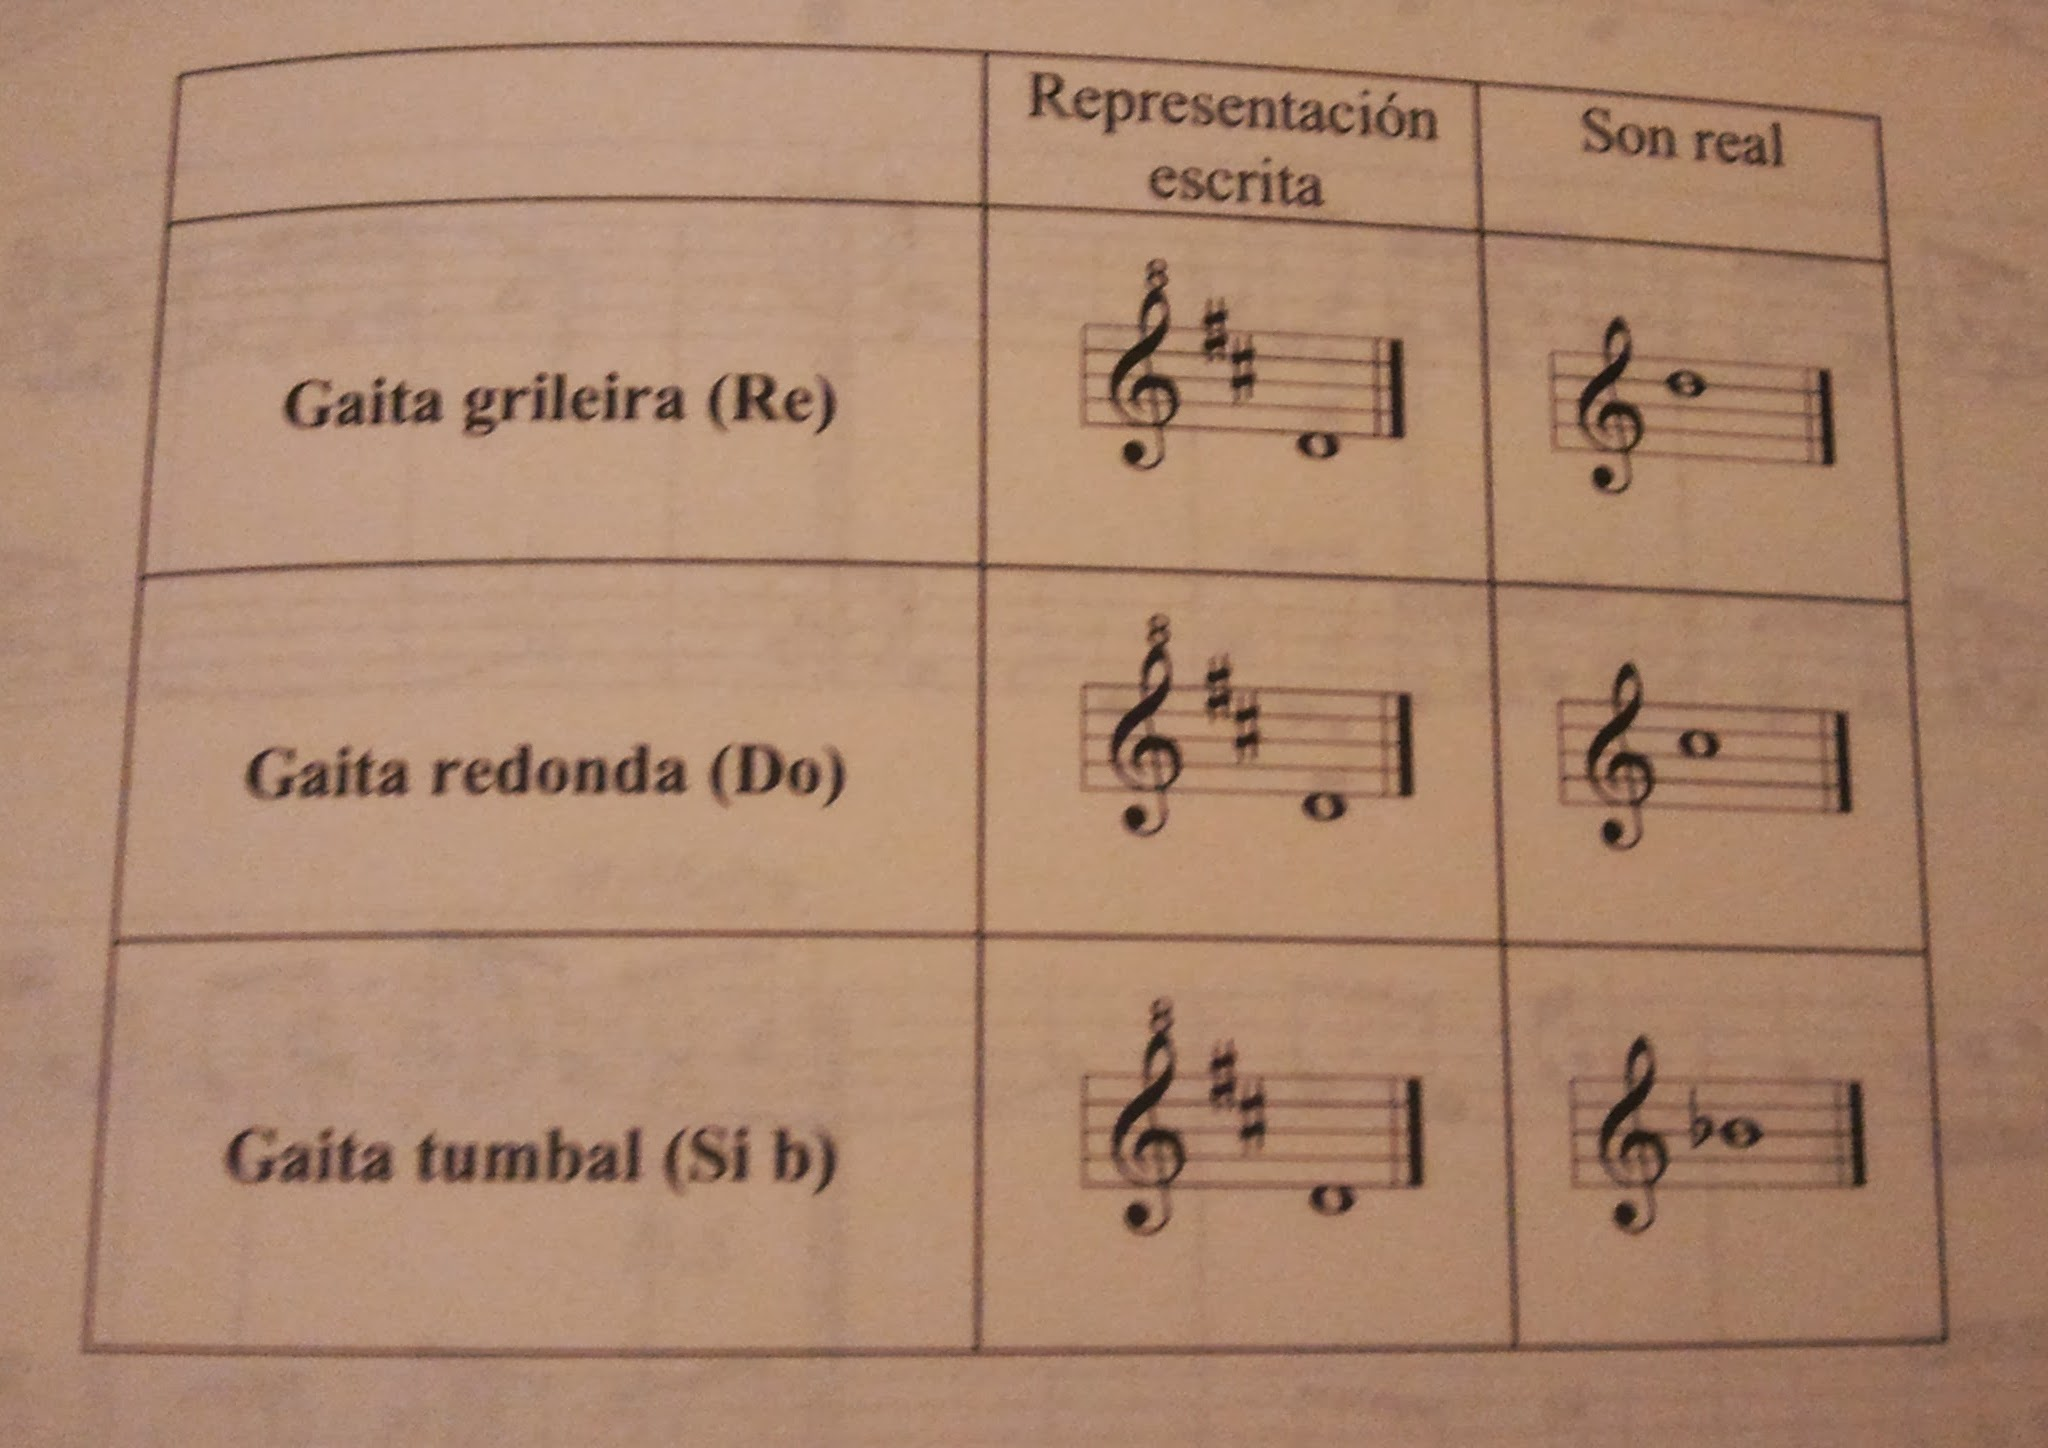
\includegraphics[scale=0.1,keepaspectratio=true]{./imagenes/bruno-villamor-tonalidade.jpg}
  % bruno-villamor-tonalidade.jpg: 2048x1448 pixel, 72dpi, 72.25x51.08 cm, bb=0 0 2048 1448
  \caption[Correspondencia entre tonalidades]{Correspondencia entre tonalidades \cite{BrunoVillamorCaderno18}}
  \label{figura:BrunoVillamorTonalidade}
 \end{figure}

\section{Estado da arte}

 \subsection{Protocolos de comunicación de instrumentos musicais}

  \subsubsection{MIDI}

  \textbf{MIDI} é o acrónimo de \textit{Musical Instrument Digital Interface}.
  Trátase dun estándar técnico que describe un protocolo, unha interface e uns
  conectores dixitais e permite que unha ampla variedade de instrumentos
  musicais electrónicos, ordenadores e outros dispositivos relacionados se
  conecten entre si \cite{WikipediaMIDI}. \\

  Unha soa conexión MIDI pode transportar ata 16 canles de información, cada
  unha das cales pode ser enrutada a un dispositivo distinto. \\

  O protocolo MIDI transporta mensaxes de eventos que especifican notación
  musical, altura e velocidade, sinais de control para parámetros coma o
  volume, o vibrato, o \textit{audio panning}, o \textit{cues} (disparadores) e
  os sinais de reloxo que establecen e sincronizan o tempo entre varios
  dispositivos. Estas mensaxes envíanse a outros dispositivos onde se controlan
  a xeración de son e outras características. Estos datos poden tamén poden
  gravarse nun dispositivo hardware ou software chamado secuenciador, que pode
  ser empregado para editar os datos e reproducilos outra vez máis tarde. \\

  A tecnoloxía MIDI foi estandarizada en 1983 por un grupo de representantes da
  industria musical e é mantida pola \textit{MIDI Manufacturers Association}
  (MMA). Todos os estándar MIDI son desenvolvidos e publicados conxuntamente
  pola MMA (USA) e polo \textit{MIDI Committee} da \textit{Association of
  Musical Electronics Industry} (AMEI) (Xapón).

   \paragraph{Historia}\mbox{}\\

   O repentino inicio dos sintetizadores analóxicos na música popular dos anos
   70 levou ós músicos a esixir máis prestacións dos seus instrumentos.
   Interconectar sintetizadores analóxicos é relativamente sinxelo xa que estes
   poden controlarse a través de osciladores de voltaxe variable. \\

   A aparición do sintetizador dixital a finais da mesma década trouxo consigo
   o problema da incompatibilidade dos sistemas que usaba cada compañía
   fabricante. Deste modo facíase necesario crear unha linguaxe común por
   enriba dos parámetros que cada marca ía xerando ó longo do desenvolvemento
   dos distintos instrumentos electrónicos postos a disposición dos
   profesionais do sector. \\

   O estándar MIDI foi inicialmente proposto nun documento dirixido á
   \textit{Audio Engineering Society} por \textit{Dave Smith}, presidente da
   compañía \textit{Sequential Circuits} en 1981. A primeira especificación
   MIDI publicouse en agosto de 1983. \\

   Cómpre aclarar que o protocolo MIDI non transmite sinais de audio, senón
   datos de eventos e mensaxes de controladores que se poden interpretar de
   maneira arbitraria, de acordo coa programación do dispositivo que os recibe.
   É dicir, o protocolo MIDI é unha especie de ``partitura'' que contén as
   instruccións en valores numéricos cando xerar unha nota de son e as
   características que debe ter; o aparato ó que se envíe dita partitura
   transformaraa en música completamente audible. \\

   Na actualidade, a gran maioría dos creadores musicais emprega o protocolo
   MIDI a fin de levar a cabo a edición de partituras e a instrumentación
   previa á gravación con instrumentos reais. Sen embargo, a perfección
   adquirida polos sintetizadores na actualidade leva á utilización de forma
   directa nas gravacións os sons resultantes do envío da partitura electrónica
   a ditos sintetizadores de última xeración.

   \paragraph{Hardware}\mbox{}\\

    \subparagraph{Dispositivos}\mbox{}\\

    Os dispositivos MIDI poden clasificarse en tres grandes categorías:

    \begin{itemize}
     \item \textbf{Controladores}. Xeran as mensaxes MIDI (activación ou
           desactivación dunha nota, variacións de ton, etc.). O controlador
           máis familiar para os músicos ten forma de teclado de piano, ó ser
           este instrumento o máis empregado á hora de compor e integrar as
           obras orquestais; sen embargo, hoxe en día contrúense todo tipo de
           instrumentos con capacidade de transmisión vía interface MIDI:
           órganos de tubos, guitarras, parches de percusión, clarinetes
           electrónicos e incluso gaitas MIDI.
     \item \textbf{Sintetizadores}. Tamén coñecidos coma unidades xeradoras de
           son ou módulos de son, reciben as mensaxes MIDI e transfórmanas en
           sinais sonoros (lembremos que o protocolo MIDI non transmite audio,
           senón paquetes de ordes en formato numérico).
     \item \textbf{Secuenciadores}. Non son máis que aparatos destinados a
           gravar, reproducir ou editar mensaxes MIDI. Poden desenvolverse ben
           en formato hardware, ben coma software de ordenador, ou ben
           incorporados nun sintetizador.
    \end{itemize}

    Estes son os tres grandes tipos de dispositivos MIDI. Aínda así, podemos
    atopar no mercado dispositivos que reúnen dúas ou tres das funcións
    descritas. Por exemplo, os órganos electrónicos dispoñen dun controlador (o
    propio teclado) e dunha unidade xeradora de son; algúns modelos tamén
    inclúen un secuenciador.

    \subparagraph{Cables e conectores}\mbox{}\\

    Un cable MIDI emprega un conector de tipo DIN de 5 pins ou contactos
    (figura \ref{figura:WikipediaConectorMIDI}).

    \begin{figure}[htbp]
     \centering
     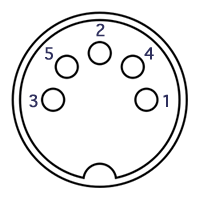
\includegraphics[scale=0.5,keepaspectratio=true]{./imagenes/wikipedia-conector-midi.png}
     % wikipedia-conector-midi.png: 200x200 pixel, 72dpi, 7.06x7.06 cm, bb=0 0 200 200
     \caption[Conector MIDI]{Conector MIDI \cite{WikipediaMIDI}}
     \label{figura:WikipediaConectorMIDI}
    \end{figure}

    A transmisión de datos só emprega un destes, o número 5. Os números 1 e 3
    reserváronse para engadir funcións nun futuro. Os restantes (2 e 4)
    empréganse -respectivamente- coma blindaxe e para transmitir unha tensión
    de +5 voltios, para asegurarse de que a electricidade flúa na dirección
    desexada. \\

    A finalidade do cable MIDI é a de permitir a transmisión dos datos entre
    dous dispositivos ou instrumentos electrónicos. Na actualidade, os
    fabricantes dos equipos económicos e, por tanto, moi populares, de empresas
    tales como Yamaha, Casio, Korg e Roland previron a substitución dos cables
    e conectores MIDI estándar polos de tipo USB, que son máis sinxelos de
    atopar no comercio e que permiten unha conexión sinxela ós ordenadores
    persoais.

    \subparagraph{Conexións}\mbox{}\\

    O sistema de funcionamento do protocolo MIDI é de tipo \textit{simplex}, é
    dicir, só pode transmitir sinais nun sentido. A dirección que toman os
    sinais é sempre desde un dispositivo 'mestre' hacia un dispositivo
    'escravo'. O primeiro xera a información e o segundo recíbea.

    \begin{figure}[htbp]
     \centering
     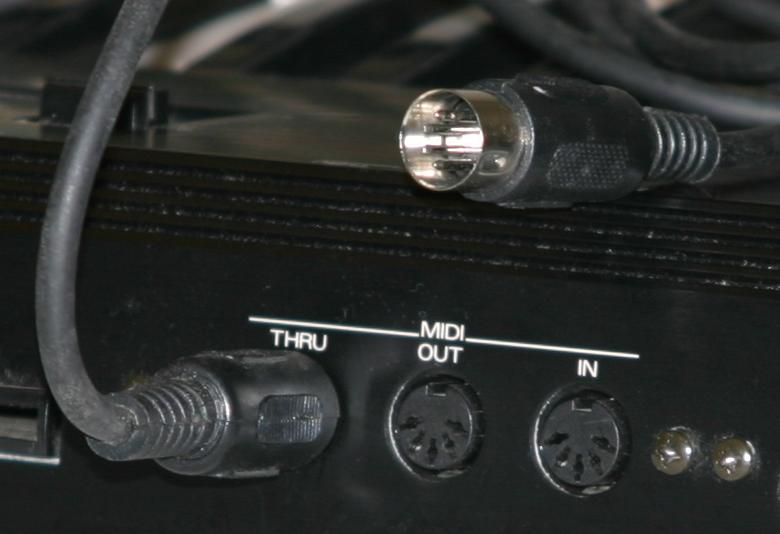
\includegraphics[scale=0.3,keepaspectratio=true]{./imagenes/wikipedia-puertos-midi.jpg}
     % wikipedia-puertos-midi.jpg: 780x534 pixel, 72dpi, 27.52x18.84 cm, bb=0 0 780 534
     \caption[Portos e cable MIDI]{Portos e cable MIDI \cite{WikipediaMIDI}}
     \label{figura:WikipediaPortosMIDI}
    \end{figure}

    Para entender ben o sistema de conexión, debemos saber que nun dispositivo
    MIDI pode haber ata tres conectores (figura
    \ref{figura:WikipediaPortosMIDI}):

    \begin{itemize}
     \item \textbf{MIDI OUT}: conector do que saen as mensaxes xeradas polo
           dispositivo mestre.
     \item \textbf{MIDI IN}: sirve para recibir mensaxes desde un dispositivo
           escravo.
     \item \textbf{MIDI THRU} tamén é un conector de saída, pero que neste caso
           envía unha copia exacta das mensaxes que entran por
           \textit{MIDI IN}.
    \end{itemize}

    O formato máis simple de conexión é o formado por un dispositivo mestre
    (por exemplo, un controlador) e un escravo (coma un sintetizador). Neste
    caso, o mestre disporá dun conector \textit{MIDI OUT} (de onde sairán as
    mensaxes MIDI xeradas), o cal deberemos de unir ó conector \textit{MIDI IN}
    no escravo. \\

    O protocolo MIDI admite a conexión dun solo mestre a varios dispositivos
    escravos en cascada. Para eses casos empregarase o conector
    \textit{MIDI THRU}, unindo o mestre cunha das unidades do modo descrito
    anteriormente. No conector \textit{MIDI THRU} desa unidad obtense unha
    copia das mensaxes MIDI que entran por \textit{MIDI IN}, polo que se
    conectamos sucesivamente o \textit{MIDI THRU} dun dispositivo co
    \textit{MIDI IN} do seguinte, obtemos o que se coñece coma unha conexión
    \textbf{Daisy Chain}. \\

    Aínda que existe a posibilidade de conectar en cascada varios dispositivos
    MIDI, é certo que existe unha limitación. As características eléctricas dos
    conectores MIDI fan a señal proclive á degradación, polo que son poucos os
    dispositivos que se poden conectar en cascada antes de notar perdas
    apreciables de información.

   \paragraph{Software}\mbox{}\\

   A especificación MIDI inclúe un aspecto software que parte desde a mesma
   organización dos bytes.

    \subparagraph{Mensaxes MIDI}\mbox{}\\

    A transmisión dos datos efectúase en serie, é dicir, un bit tras outro, de
    maneira asíncrona, o que obriga a agregar un bit de inicio e outro de
    parada. \\
  
    Para clarificar o dito, pódese dicir sinxelamente que unha transmisión
    asíncrona de datos dase cando un receptor non sabe cando virá o seguinte
    dato, polo que se atopa en estado de constante espera, xa sexa en nivel
    alto ou baixo, ata que se produza un cambio de estado que indique o inicio
    dunha nova mensaxe. \\

    Este primeiro bit debe ser sempre o mesmo, para que sexa sempre diferente ó
    estado ``por defecto'', así que este bit non pode formar parte do byte
    recibido. A este bit que serve para indicar a chegada dun dato e permite ó
    dispositivo receptor prepararse para a cadea de bits que vén despois,
    coñéceselle como ``bit de inicio''. Na especificación MIDI, a entrada
    atópase nun estado alto por defecto, así que o bit de inicio é un 0. \\

    O bit de parada serve para dar tempo ó dispositivo receptor para decidir
    que facer coa información unha vez recibida. No caso do protocolo MIDI,
    este bit é sempre o 1. \\

    A velocidade de transmisión do protocolo MIDI definiuse en 31.250 baudios,
    polo que só deben transcorrer 32 microsegundos entre un bit e o seguinte;
    nin máis, nin menos. Tamén se esixe que a orde de envío dos bits de cada
    byte sexa LSB, é dicir, o de menos peso primeiro. \\

    Na especificación MIDI existen dous tipos de bytes: de estado -status byte-
    e de información -data byte-. \\

    Estes diferéncianse polo primeiro bit: se é un 1, será un byte de estado e
    se é un 0, é un byte de datos. \\

    Ó xerar unha mensaxe MIDI, por norma xeral, sempre enviamos un byte de
    estado, que pode estar seguido de certa cantidade de bytes de datos. Por
    exemplo, podemos enviar unha primeira mensaxe de estado ``activar nota'',
    seguida dun byte de datos informando que nota é a que se activa. Nalgunhas
    ocasións e segundo o dispositivo MIDI do que trate, pode ocorrer que se
    omita o byte de estado se é idéntico ó anterior. \\

    Por exemplo, se tocamos a tecla Do central dun teclado MIDI mandaría:

    \begin{itemize}
     \item 1001xxxx (Note on)
     \item 00111100 (Valor 60 que corresponde á nota Do central "C3")
     \item 0xxxxxxx (A velocidade ou intensidade co que se foi apretada a
           tecla)
    \end{itemize}

    Pero ó soltala, pode omitir o byte de estado e apagala ``por volume'' no
    canto de apagala cunha mensaxe de ``Note off'' (1000xxxx). É dicir,
    transmitiría só os dous seguintes bytes:

    \begin{itemize}
     \item 00111100 (Valor 60 que corresponde á nota Do central "C3")
     \item 00000000 (A velocidade cero, que indica que ten que deixar de soar
           esa nota)
    \end{itemize}

    Omitindo así o byte de estado. É máis, se novamente pulsamos a mesma tecla
    outra vez, volvería omitir o byte de estado. \\

    Á súa vez, as mensaxes de estado divídense en dous grupos: mensaxes de
    canle e mensaxes de sistema. As mensaxes de canle envíanse a un dispositivo
    específico, mentres que as mensaxes de sistema son recibidas por todos os
    dispositivos. \\

    Na seguinte táboa (táboa \ref{tabla:WikipediaMensaxesMIDI}) amósanse todas
    as mensaxes dispoñibles. \\

    \begin{table}[htbp]
     \centering
     \begin{tabular}{|l|l|}
      \hline
      \textbf{Byte estado} & \textbf{Descrición} \\
      \hline
      1000cccc & Desactivación de nota \\
      \hline
      1001cccc & Activación de nota \\
      \hline
      1010cccc & Postpulsación polifónica \\
      \hline
      1011cccc & Cambio de control \\
      \hline
      1100cccc & Cambio de programa \\
      \hline
      1101cccc & Postpulsación monofónica de canle \\
      \hline
      1110cccc & Pitch \\
      \hline
      11110000 & Mensaxe exclusiva do fabricante \\
      \hline
      11110001 & Mensaxe de trama temporal \\
      \hline
      11110010 & Punteiro posición de canción \\
      \hline
      11110011 & Selección de canción \\
      \hline
      11110100 & Indefinido \\
      \hline
      11110101 & Indefinido \\
      \hline
      11110110 & Requirimento de entoación \\
      \hline
      11110111 & Fin de mensaxe exclusiva \\
      \hline
      11111000 & Reloxo de temporización \\
      \hline
      11111001 & Indefinido \\
      \hline
      11111010 & Inicio \\
      \hline
      11111011 & Continuación \\
      \hline
      11111100 & Parada \\
      \hline
      11111101 & Indefinido \\
      \hline
      11111110 & Espera activa \\
      \hline
      11111111 & Reseteo do sistema \\
      \hline
     \end{tabular}
     \caption{Mensaxes MIDI}
     \label{tabla:WikipediaMensaxesMIDI}  
    \end{table}
  
    Os primeiros bytes, cuxos últimos catro bits están marcados como ``cccc'',
    refírense a mensaxes de canle; o resto de bytes son mensaxes de sistema.

    \subparagraph{Canles MIDI}\mbox{}\\

    Como se comentou con anterioridade, o protocolo MIDI está pensado para
    comunicar un único controlador con varios sintetizadores (cada un dos cales
    pode ter un ou varios instrumentos sintetizados que se desexan utilizar),
    todo por un mesmo medio de transmisión. É dicir, tódolos dispositivos á
    cadea MIDI reciben tódalas mensaxes xeradas desde o controlador. Isto fai
    necesario un método para diferenciar cada un dos instrumentos. Este método
    é o que se denomina \textbf{canle}. \\

    O protocolo MIDI pode direccionar ata 16 canles (tamén chamadas voces ou
    instrumentos); por ilo, ó instalar o sistema MIDI será necesario asignar un
    número de canle para cada dispositivo.

    \subparagraph{General MIDI}\mbox{}\\

    O protocolo MIDI permite seleccionar o son dun instrumento a través dunha
    mensaxe de cambio de programa, pero non hai garantía de que dous
    dispositivos teñan o mesmo son para un programa determinado. O programa 0
    pode corresponderse cun piano nun dispositivo e cunha frauta noutro. \\

    O estándar \textbf{General MIDI} (GM) aprobouse en 1991 e estableceu e
    estandarizou un banco de sons que permite que un ficheiro MIDI estándar
    creado por un dispositivo soe de maneira similar cando sexa reproducido
    noutro. \\

    GM especifica un banco de 128 sons agrupados en 16 familias de 8
    instrumentos relacionados e asigna un número de programa específico a cada
    instrumento. Os dispositivos compatibles con GM deben ofrecer polifonías de
    ata 24 notas. Calquera cambio de programa que se faga seleccionará o mesmo
    son de instrumento en calquera dispositivo compatible con GM. \\

    O estándar GM elimina a variación no mapeo de notas. GM especifica que a
    nota número 69 se corresponde coa nota A440 (La a 440 Hz, que é a nota que
    se toma como referencia para afinar), o que fai que o Do central se fixe
    como nota número 60. \\

    No estándar GM, a gaita forma parte da familia de instrumentos étnicos
    (105-112) e corresponde ó número 109.

    \subparagraph{Modos MIDI}\mbox{}\\

    Dentro do sistema MIDI decidiuse crear unha serie de diferentes
    \textbf{modos} de funcionamento, cada un con certas características. Antes
    de velos, debemos diferenciar os seguintes conceptos:

    \begin{itemize}
     \item \textit{Monofónico}. Un instrumento monofónico só pode reproducir
           unha nota simultaneamente. É dicir, para reproducir unha nova nota
           debe deixar de soar primeiro a nota anterior. Por exemplo, os
           instrumentos de vento son monofónicos, xa que só reproducen un único
           son cada vez.
     \item \textit{Polifónico}. Un instrumento polifónico pode reproducir
           varias notas simultaneamente. Un exemplo é o piano, que pode formar
           acordes por medio de facer soar dúas ou máis notas á vez.
    \end{itemize}

    Aclarados estes conceptos, podemos resumir os modos MIDI na seguinte táboa
    (táboa \ref{tabla:WikipediaModosMIDI}). \\

    \begin{table}[htbp]
     \centering
     \begin{tabular}{|l|l|l|}
      \hline
      \textbf{Número} & \textbf{Nome} & \textbf{Descrición} \\
      \hline
      1 & Omni on / poly & Funcionamento polifónico sen información de canle \\
      \hline
      2 & Omni on / mono & Funcionamento monofónico sen información de canle \\
      \hline
      3 & Omni off / poly & Funcionamento polifónico con múltiples canles \\
      \hline
      4 & Omni off / mono & Funcionamento monofónico con múltiples canles \\
      \hline
     \end{tabular}
     \caption{Modos MIDI}
     \label{tabla:WikipediaModosMIDI}  
    \end{table}

    O modo \textit{Omni On} significa que un dispositivo responderá en tódalas
    canles. Estas configuracións resérvanse para configuracións onde só
    empreguemos un instrumento. \\

    No modo \textit{Onmi Off} polifónico (modo 3), un dispositivo só responde a
    unha única canle MIDI predeterminada. \\

    No modo \textit{Onmi Off} monofónico (modo 4), cada voz pode ser asignada á
    súa propia canle MIDI.

  \subsubsection{OSC}

  \textbf{Open Sound Control} (OSC) \cite{OSC} é un formato de contido para a
  comunicación entre ordenadores, sintetizadores de son e outros dispositivos
  multimedia optimizados para as tecnoloxías de rede modernas. \\

  Ademais de aportar os beneficios da tecnoloxía moderna para o mundo dos
  instrumentos musicais electrónicos, as vantaxes de OSC inclúen a
  interoperabilidade, a precisión, a flexibilidade e unha maior organización e
  documentación.

  \paragraph{Motivación}\mbox{}\\

  OSC é un formato de contido desenvolvido no
  \textit{Center for New Music and Audio Technologies} (CNMAT) da
  \textit{University of California}, Berkeley, por \textit{Adrian Freed} e
  \textit{Matt Wright}, comparable a formatos coma XML, WDDX ou JSON. \\

  Orixinalmente foi pensado para compartir información musical (xestos,
  parámetros e secuencias de notas) entre instrumentos musicais (especialmente
  instrumentos musicais electrónicos coma os sintetizadores), ordenadores e
  outros dispositivos multimedia. \\

  OSC é usado normalmente como alternativa ó estándar MIDI de 1983 naqueles
  casos nos que se precisa maior resolución e parámetros musicais máis
  elaborados. \\

  As mensaxes OSC envíanse normalmente a través de Internet ou de redes
  persoais ou dun estudo usando UDP/IP e Ethernet. \\

  OSC ofrece a músicos e desenvolvedores unha maior flexibilidade nos tipos de
  datos que se poden enviar a través de cable, o que permite que novos tipos de
  aplicacións se poidan comunicar a alto nivel entre elas.

  \paragraph{Características}\mbox{}\\

  \begin{itemize}
   \item Esquema de nomeado simbólico, dinámico e ampliable.
   \item Datos numéricos simbólicos e de alta resolución.
   \item Linguaxe de tipo \textit{pattern matching} para especificar múltiples
         receptores dunha única mensaxe.
   \item Etiquetas temporais de alta resolución.
   \item Conxuntos de mensaxes cuxos efectos poden simultanearse.
  \end{itemize}

  Hai ducias de implementacións de OSC, incluíndo son en tempo real e entornos
  de procesamento de medios, ferramentas web interactivas, sintetizadores
  software e unha longa lista de linguaxes de programación e dispositivos
  hardware. \\

  OSC emprégase amplamente en controladores musicais experimentais e
  incorporouse en múltiples productos comerciais e open source.

  \paragraph{Deseño}\mbox{}\\

  As mensaxes OSC constan de:

  \begin{itemize}
   \item Un patrón de dirección: os patróns de direccións forman un espacio de
         nomes xerárquico, herdado dos sistemas de ficheiros GNU/Linux e das
         URL.
   \item Unha cadea que contén etiquetas de tipos: son cadeas que conteñen unha
         representación dos tipos de datos dos argumentos en forma de etiquetas.
   \item Argumentos: represéntanse en formato binario con aliñamento de 4
         bytes. Os tipos soportados son:
         \begin{itemize}
          \item Enteiros sen signo de 32 bits en complemento a dous.
          \item Números en punto flotante de 32 bits en formato IEEE.
          \item Arrays de datos codificados de 8 bits rematados nun punteiro a nulo.
          \item Blobs de tamaño arbitrario (audio ou vídeo).
         \end{itemize}
   \item Unha etiqueta temporal opcional.
  \end{itemize}

  \subsubsection{MIDI vs OSC}

  As vantaxes de OSC sobre MIDI son principalmente a conectividade a través de
  Internet, a resolución dos tipos de datos e a facilidade de especificar unha
  ruta simbólica. \\

  OSC pode ser enviado a través de conexións Ethernet a velocidades de banda
  larga, pero é pouco adecuado como solución única para un estudo de gravación,
  dado que a día de hoxe non conta co apoio da maioría do hardware e software
  máis empregados. \\

  O aumento de tamaño das mensaxes OSC en comparación coas mensaxes MIDI fano
  unha solución impracticable para moitos dispositivos móbiles e as súas
  alabadas vantaxes de velocidade sobre MIDI desaparecen cando ambos transmiten
  polo mesmo medio. \\

  OSC non é propietario, pero non é mantido por ningunha organización
  estandarizadora. \\

  Por todos estes motivos, decidiuse usar o protocolo MIDI para o proxecto,
  dado que se adapta moito mellor ás esixencias do mesmo.
  
  \subsubsection{Alternativas actuais}
  
  Pasou xa moito tempo dende que no 1983 se anunciara MIDI coma novo protocolo
  de comunicación entre instrumentos musicais dixitais heteroxéneos. E se
  botamos a vista atrás e comparamos co estado actual, a verdade é que non
  cambiou moito. \\
  
  Certamente resulta incrible que un sistema con tantos anos ás costas e sen
  apenas modificacións siga sendo empregado tan profusamente a día de hoxe. \\
  
  Aínda que houbo un intento de actualizar o protocolo alá polo 2013
  de nome \textit{HD-MIDI} \cite{HDMIDI} e que prometía un maior rango de
  canles, maior rango e resolución de datos, transporte sobre redes con e sen
  fíos e incluso soporte de controladores de guitarra, a realidade é que fóra
  duns poucos prototipos presentados por fabricantes, non se volveu saber máis
  nada del. \\
  
  Houbo tamén unha corrente \textit{revival} alternativa en favor de OSC, o
  conto non pasou de soporte esporádico para algún software recoñecido de
  sistemas MacOs, pero sen repercusión real. \\
  
  Polo que parece, tal e como comenta \textit{Nik Reiman} \cite{NikReiman}, MIDI
  non vai ir a ningures, dado que é tan simple e universal, que calquera
  aplicación ou hardware que realices empregando MIDI non ten un alto risco de
  obsolescencia por dito motivo.

 \subsection{Gaitas MIDI}

 Fóra do que poida parecer a priori, o estado da arte en canto a gaitas MIDI se
 refire é moi amplo e variado, polo que estudialo na súa totalidade
 describíndoo en profundidade escapa do ámbito deste proxecto, aínda que se
 inclúen as referencias principais necesarias para que o lector interesado
 poida profundizar no tema. \\

 Curiosamente, os mellores exemplos son os que teñen entre os seus destinos o
 mercado galego, polo que nos centraremos case exclusivamente nestes modelos,
 ordenados por cantidade de funcionalidades e, por tanto, tamén por precio de
 venda.

 Así mesmo, comentaranse as carencias detectadas en cada exemplo, as cales se
 tratarán de subsanar no producto obtido ó final do presente proxecto.

  \subsubsection{Master Gaita}

  \begin{figure}[htbp]
   \centering
   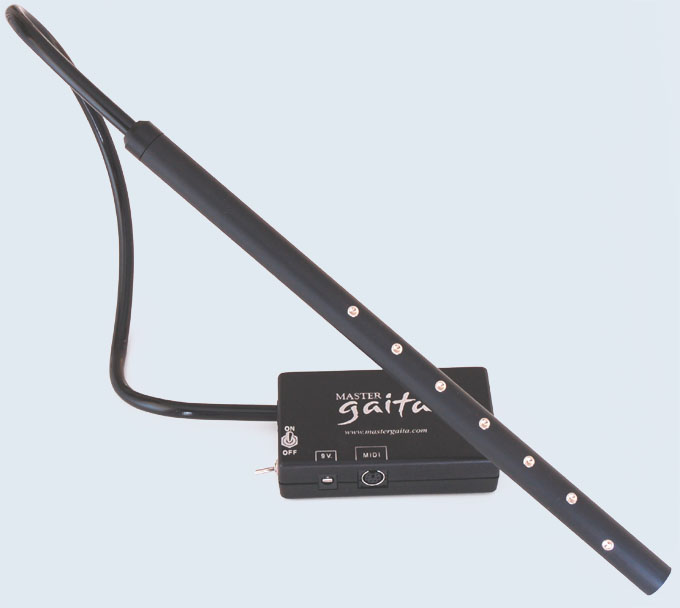
\includegraphics[scale=0.2,keepaspectratio=true]{./imagenes/master-gaita.jpg}
   % master-gaita.jpg: 680x608 pixel, 72dpi, 23.99x21.45 cm, bb=0 0 680 608
   \caption[Master Gaita]{Master Gaita \cite{MasterGaita}}
   \label{figura:MasterGaita}
  \end{figure}

  É un controlador MIDI montado nun tubo de PVC con nove dispositivos táctiles.
  Un cable semiríxido e unha caixa (onde se aloxa a circuitería) serven de
  punto de apoio a modo de fol para suxeitar o punteiro. \\

  \textbf{Características:}

  \begin{itemize}
   \item Cinco dixitacións cromáticas seleccionables (galega, asturiana,
         escocesa, francesa e estendida de 2,5 oitavas).
   \item Compatible con outras gaitas como a de Boto, Sac de Gemecs e Xeremía.
   \item Cambio a calquera tonalidade e oitava.
   \item Control independente do roncón e ronqueta, permitindo afinar esta
         última na tónica ou na dominante.
   \item Catro programas sonoros seleccionables con dous instrumentos cada un.
   \item Acompañamento automático a dúo por terceiras superiores ou inferiores.
   \item Conexión directa a un ordenador empregando un \textit{Game port}.
   \item Conexión a unha cadea MIDI estándar co cable MIDI incorporado.
   \item Posibilidade de conexión mediante cable conversor USB-MIDI (non
         incluído).
   \item Auto-apagado tras 2 ou 10 minutos (a escoller) de inactividade.
   \item Suxección similar á dunha gaita.
   \item Alimentación con pila de 9V ou fonte externa.
   \item Manual de usuario e conxunto de samples.
  \end{itemize}

  \textbf{Carencias detectadas:}

  \begin{itemize}
   \item As dixitacións son limitadas.
   \item Non ten conexión directa cun ordenador moderno. Precisa dun conversor,
         o que implica maiores retardos.
   \item Non dispón de conexión sen fíos.
   \item Precisa de alimentación separada da conexión de datos.
   \item A suxección aínda que similar á dunha gaita, é de todo menos cómoda.
   \item Non se pode acoplar a unha gaita.
   \item A forma do punteiro é cilíndrica, non cónica como a dun punteiro real,
         o que xera rechazo.
   \item Os sensores sobresaen do punteiro, o que fai perder a sensación de
         burato dun punteiro real.
  \end{itemize}

  \textbf{Prezos:}

  \begin{itemize}
   \item Master Gaita: 275 euros (IVE n.i.).
  \end{itemize}

 \subsubsection{Technopipes}

  \begin{figure}[htbp]
   \centering
   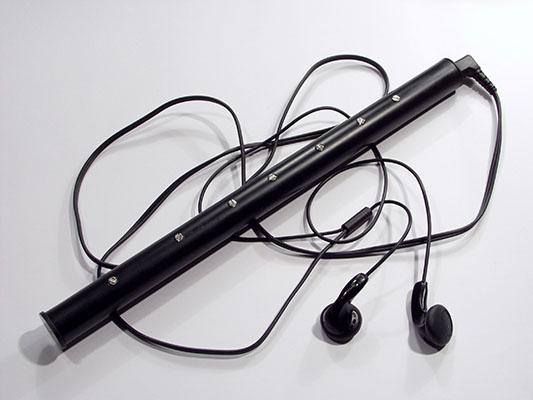
\includegraphics[scale=0.3,keepaspectratio=true]{./imagenes/technopipes.jpg}
   % technopipes.jpg: 533x400 pixel, 72dpi, 18.80x14.11 cm, bb=0 0 533 400
   \caption[Technopipes]{Technopipes \cite{Technopipes}}
   \label{figura:Technopipes}
  \end{figure}

  Controlador MIDI montado nun tubo de PVC con posibilidade de acoplarlle un
  accesorio de apoio (non incluído). \\

  \textbf{Características:}

  \begin{itemize}
   \item Dixitacións galega, asturiana e escocesa.
   \item Dispón de bordóns.
   \item Soporta 4 tonalidades: La, Sib, Do e Re.
   \item Portátil.
   \item Conta con saída MIDI (cable incluído).
   \item Conta con saída de audio para auriculares (non incluídos).
   \item Funcionamento a pilas. Ata 10 horas de autonomía.
   \item Sensibilidade axustable.
   \item Conta con metrónomo.
   \item Pode gravar e reproducir o que se toca.
   \item Conta cun conxunto de samples.
   \item Reconfigurable desde o propio controlador.
  \end{itemize}

  \textbf{Carencias detectadas:}

  \begin{itemize}
   \item As dixitacións son limitadas.
   \item Non ten conexión directa cun ordenador moderno. Precisa dun conversor,
         o que implica maiores retardos.
   \item Non dispón de conexión sen fíos.
   \item Non se pode acoplar a unha gaita.
   \item A forma do punteiro é cilíndrica, non cónica como a dun punteiro real,
         o que xera rechazo.
   \item Os sensores sobresaen do punteiro, o que fai perder a sensación de
         burato dun punteiro real.
   \item Autonomía limitada.
  \end{itemize}

  \textbf{Prezos:}

  \begin{itemize}
   \item Technopipes: 365 euros (IVE inc.).
   \item Soporte: 26 euros (IVE inc.).
  \end{itemize}

  \subsubsection{ePipe}

  \begin{figure}[htbp]
   \centering
   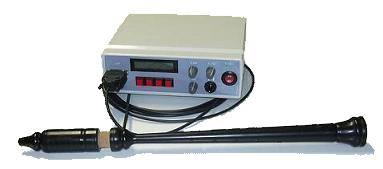
\includegraphics[scale=0.9,keepaspectratio=true]{./imagenes/epipe.jpg}
   % epipe.jpg: 383x169 pixel, 96dpi, 10.13x4.47 cm, bb=0 0 287 127
   \caption[ePipe]{ePipe \cite{ePipe}}
   \label{figura:ePipe}
  \end{figure}

  Consta dun punteiro MIDI e dun conversor de analóxico-dixital de grandes
  proporcións. Existe a opción de disimular o conversor dentro dun
  amplificador. \\

  \textbf{Características:}

  \begin{itemize}
   \item Dixitacións galega e asturiana.
   \item Catro conxuntos de samples.
   \item Tonalidades: La, Sib, Si, Do, Do\# e Re.
   \item Controis independentes de volume.
   \item Conta con sensor de presión regulable.
   \item Sensibilidade regulable.
   \item Conectores MIDI completos.
   \item Saída para auriculares.
  \end{itemize}

  \textbf{Carencias detectadas:}

  \begin{itemize}
   \item As dixitacións son limitadas.
   \item As tonalidades son limitadas.
   \item Non ten conexión directa cun ordenador moderno. Precisa dun conversor,
         o que implica maiores retardos.
   \item Non dispón de conexión sen fíos.
   \item Os sensores son pouco convencionais e propensos a erros.
   \item As dimensións do conversor analóxico-dixital son desproporcionadas.
  \end{itemize}

  \textbf{Prezos:}

  \begin{itemize}
   \item ePipe 15: 645 euros (IVE n.i.).
   \item ePipe 25 (amplificador): 745 euros (IVE n.i.).
  \end{itemize}

  \subsubsection{Hevia Electronic Bagpipe}

  \begin{figure}[htbp]
   \centering
   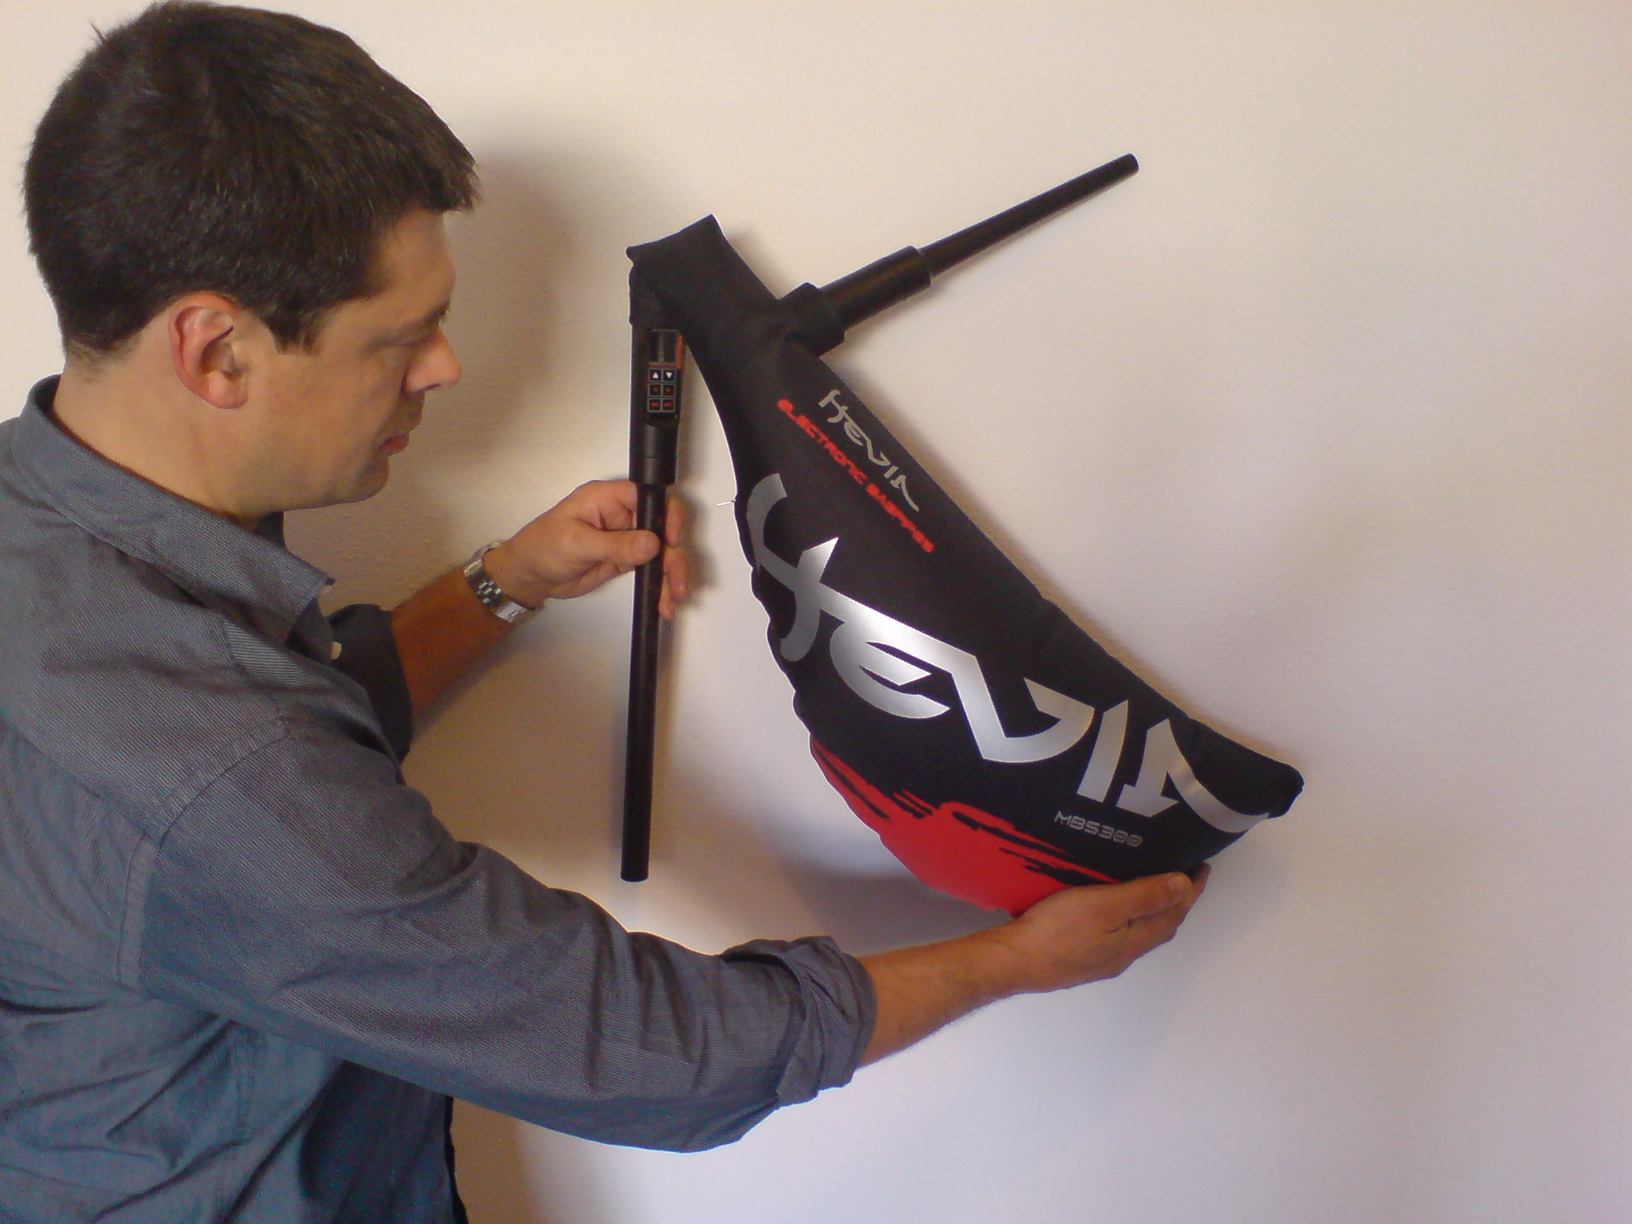
\includegraphics[scale=0.1,keepaspectratio=true]{./imagenes/hevia-mbs-300.jpg}
   % hevia-mbs-300.jpg: 1632x1224 pixel, 72dpi, 57.57x43.18 cm, bb=0 0 1632 1224
   \caption[Hevia MBS 300]{Hevia MBS 300 \cite{HeviaMBS300}}
   \label{figura:HeviaMBS300}
  \end{figure}

  Controlador MIDI que simula unha gaita case completa (sen bordóns reais). O
  modelo que se analiza aquí é o MBS-300, existindo actualmente un modelo máis
  recente, o MBS-250, que é máis barato, pero tamén vén con funcionalidades
  recortadas, o que non nos interesa para a avaliación de características. \\

  \textbf{Características:}

  \begin{itemize}
   \item Sensión de presión regulable.
   \item Dispón de bordóns.
   \item Dixitacións totalmente configurables.
   \item Oitavas totalmente configurables.
   \item Transporte de tonalidade.
   \item Soporta glissando e vibrato.
   \item Reconfigurable desde o propio controlador.
   \item Módulo bluetooth (opcional). Alcance 100m.
  \end{itemize}

  \textbf{Carencias detectadas:}

  \begin{itemize}
   \item As dixitacións son limitadas.
   \item As tonalidades son limitadas.
   \item Non se pode acoplar a unha gaita convencional.
   \item A forma do punteiro é cilíndrica, non cónica como a dun punteiro real,
         o que xera rechazo.
   \item Os sensores exactamente ó mesmo nivel do punteiro, o que dificulta a
         localización dos mesmos.
   \item A conexión bluetooth con esa potencia ten un alto consumo, o que
         merma a súa autonomía ostensiblemente.
  \end{itemize}

  \textbf{Prezos:}

  \begin{itemize}
   \item MBS-300: 1.999 euros (IVE n.i.).
   \item Módulo bluetooth: 127 euros (IVE n.i).
   \item Módulo externo de son: 170 euros (IVE n.i.).
  \end{itemize}

  \subsubsection{OpenPipe}
 
  \begin{figure}[htbp]
   \centering
   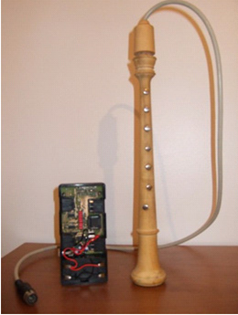
\includegraphics[scale=0.7,keepaspectratio=true]{./imagenes/openpipe.png}
   \caption[OpenPipe]{OpenPipe \cite{OpenPipe}}
   \label{figura:OpenPipe}
  \end{figure}

  Punteiro MIDI non comercial con formato de punteiro convencional e conexión
  vía porto MIDI desenvolvido baixo os principios do software libre. \\

  \textbf{Características:}

  \begin{itemize}
   \item Sensibilidade regulable.
   \item Dispón de bordóns.
   \item Dixitacións totalmente configurables.
   \item Transporte de tonalidade.
   \item Conexión mediante porto MIDI e conversor MIDI-USB.
  \end{itemize}

  \textbf{Carencias detectadas:}

  \begin{itemize}
   \item Non se pode acoplar a unha gaita convencional, aínda que sería
         facilmente modificable para ilo.
   \item Os sensores sobresaen do punteiro, o que fai perder a sensación de
         burato dun punteiro convencional.
   \item Un pouco curto en canto a funcionalidade, pero máis que suficiente
         para un PFC.
  \end{itemize}
